\chapter{拟范畴的解析理论}\label{ch:analytic-theory-of-quasi-categories}


在本最后一个附录中，我们的目标是证明：拟范畴的综合理论与由 André Joyal、%
Jacob Lurie 以及许多其他人所开创的解析理论是相容的。在 F.1 节中，我们证明%
拟范畴中\trTerminal{}\trElement{}的综合定义与解析定义之间的等价。在 F.2 节中，%
我们将这些结果扩充到取值于拟范畴的任意形状\trDiagram{}之\trLimit{}的综合%
定义与解析定义之间的等价。

在 F.3 节中，我们对拟范畴之间容许\trRightAdjoint\trRightInverse{}的那些%
\trIsofibration{}给出了一个新的解析刻画。这一刻画在 F.4 节中用于比较拟范畴的%
\trCartesianFibration{}与\trCartesianArrow{}的综合定义和解析定义。最后，在 F.5 节中，%
我们证明\trAdjunction{}的综合定义与解析定义彼此一致，尽管二者的形态大不相同。


\providecommand{\sSet}{s\mathcal{S}et}%

\section{始元素与终元素}\label{sec:f-initial-and-terminal-elements}

本节中，我们完成\cref{dig:terminal-elements-quasi-category}中概述的论证，%
证明拟范畴中\trTerminal{}\trElement{}的综合定义与 Joyal \cite[4.1]{bib61}%
最先引入的解析定义相一致。我们证明\trTerminal{}\trElement{}的四个综合定义%
——(i) 最先出现于\cref{def:initial-terminal-element}中的那个；(ii) 即%
\cref{lem:minimal-data}的那个；(iii) 作为\cref{prop:terminal-initial-trivial-fibration}%
出现的那个；以及 (iv) 文献中常见的那个（见例如 \cite{bib88}）——与%
\trTerminal{}\trElement{}的两个解析定义 (v) 与 (vi) 之间的等价；Joyal 已证明%
后二者彼此等价 \cite[4.2]{bib61}。

\begin{proposition}\label{prop:terminal-element-equivalences}
对于\trQuasiCategory{} $A$ 与\trElement{} $t\colon 1\to A$，以下条件等价：
\begin{enumerate}[label=(\roman*)]
\item \trElement{} $t$ 定义了唯一\trFunctor
\begin{center}
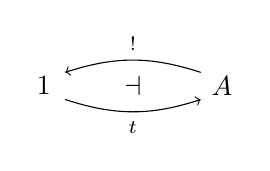
\begin{tikzpicture}[x=1.4em,y=1.4em]
  \node (One) at (0,0)   {$1$};
  \node (A)   at (4.6,0) {$A$};
  \draw[->] (4.05,0.35) to[bend right=18] node[above]{$\scriptstyle !$} (0.55,0.35);
  \node at (2.3,0) {$\dashv$};
  \draw[->] (0.55,-0.35) to[bend right=18] node[below]{$\scriptstyle t$} (4.05,-0.35);
\end{tikzpicture}
\end{center}
的\trRightAdjoint{}。
\item 存在一个\trNaturalTransformation
\begin{center}
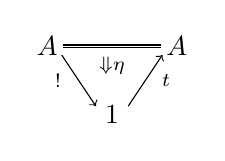
\begin{tikzpicture}[x=1.3em,y=1.3em]
  \node (L) at (0,0)    {$A$};
  \node (R) at (3.6,0)  {$A$};
  \draw[double] (0.45,0) -- (3.15,0);
  \node at (1.8,-0.55) {$\scriptstyle\Downarrow\eta$};
  \node (B) at (1.8,-1.9) {$1$};
  \draw[->] (0.4,-0.24) -- (1.35,-1.66);
  \node at (0.3,-0.95) {$\scriptstyle !$};
  \draw[->] (2.25,-1.66) -- (3.2,-0.24);
  \node at (3.3,-0.95) {$\scriptstyle t$};
\end{tikzpicture}
\end{center}
使得其分量 $\eta t$ 是一个\trIsomorphism{}。
\item 定义域投影\trFunctor
\begin{center}
$\mathrm{Hom}_{A}(A,t)\xrightarrow[\sim]{\ p_{0}\ }A$
\end{center}
定义一个\trTrivialFibration{}。
\item 对任何\trElement{} $a\colon 1\to A$，\trMappingSpace{}
$\mathrm{Hom}_{A}(a,t)$ 是\trContractible{}。
\item 投影\trFunctor
\begin{center}
$A_{/t}\xrightarrow{\ \sim\ }A$
\end{center}
——其定义域是 $A$ 在 $t$ 之上的切片——是一个\trTrivialFibration{}。
\item $A$ 中末顶点为 $t$ 的任何\trSphere{}都容许一个填充体：
\begin{center}
\begin{tikzpicture}[x=1.9em,y=1.4em]
  \node (o)  at (0,1.3)    {$1$};
  \node (pd) at (3.4,1.3)  {$\partial\Delta[n]$};
  \node (a)  at (7.4,1.3)  {$A$};
  \node (dn) at (3.4,-1.5) {$\Delta[n]$};
  \draw[->] (o) -- node[below]{$\scriptstyle\{n\}$} (pd);
  \draw[->] (pd) -- (a);
  \draw[->] (o) to[bend left=28] node[above,pos=0.5]{$\scriptstyle t$} (a);
  \draw[right hook->] (3.4,0.95) -- (3.4,-1.15);
  \draw[->,dashed] (3.75,-1.3) -- (7.0,1.0);
\end{tikzpicture}
\end{center}
\end{enumerate}
当这些条件成立时，$t$ 定义了 $A$ 的一个\textbf{\trTerminal{}\trElement}。
\end{proposition}

\begin{proof}
拆解 (i)：要定义\trAdjunction{} $!\dashv t$，所须的全部数据不过是一个%
\trUnit{}\trNaturalTransformation{} $\eta\colon\mathrm{id}_{A}\Rightarrow t!$，%
使得其分量 $\eta t=\mathrm{id}_{t}$ 为恒等。但正如\cref{lem:minimal-data}所%
证明的，若 $\eta t$ 可逆，则它必为恒等。这就证明了 (i) 与 (ii) 的等价性。

\cref{prop:terminal-initial-trivial-fibration}在任何\trInfinityCosmos{}中
建立了 (i) 与 (iii) 的等价性。由\cref{cor:discrete-cartesian-trivial-contractible}与%
\cref{cor:domain-projection-from-element}，定义域投影\trFunctor{}是一个%
\trTrivialFibration，当且仅当其诸\trFiber{} $\mathrm{Hom}_{A}(a,t)$ 是%
\trContractible{}，这就证明了 (iii) 与 (iv) 的等价性。

由\cref{cor:slice-cone-point}，对\trQuasiCategory{}中的任何顶点 $t$，在%
\cref{prop:join-slice-adjunction}之切片构造的典范投影与定义域投影%
\trIsofibration{}之间存在一个\trEquivalence
\begin{center}
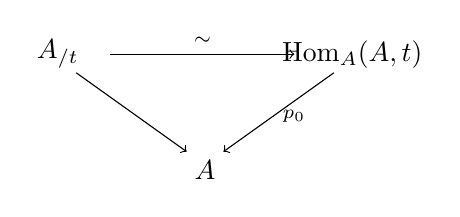
\begin{tikzpicture}[x=1.9em,y=1.5em]
  \node (at) at (0,1.3)    {$A_{/t}$};
  \node (h)  at (5.6,1.3)  {$\mathrm{Hom}_{A}(A,t)$};
  \node (a)  at (2.8,-1.5) {$A$};
  \draw[->] (1.0,1.3) -- node[above]{$\scriptstyle\sim$} (4.5,1.3);
  \draw[->] (0.35,0.85) -- (2.45,-1.05);
  \draw[->] (5.25,0.85) -- node[right,pos=0.55]{$\scriptstyle p_{0}$} (3.15,-1.05);
\end{tikzpicture}
\end{center}
于是，由\trTwoOfThreeProperty，二者之中一条\trIsofibration{}是一个%
\trEquivalence，当且仅当另一条亦然，这就证明了 (iii) 与 (v) 的等价性。

依\cref{def:trivial-fibration}，投影 $A_{/t}\twoheadrightarrow A$ 是一个%
\trTrivialFibration，当且仅当对一切 $n\ge 0$，如下右提升性质成立
\begin{center}
\begin{tikzpicture}[x=1.9em,y=1.5em]
  \node (pd) at (0,1.3)    {$\partial\Delta[n]$};
  \node (at) at (4.4,1.3)  {$A_{/t}$};
  \node (dn) at (0,-1.5)   {$\Delta[n]$};
  \node (a)  at (4.4,-1.5) {$A$};
  \draw[->] (1.0,1.3) -- node[above]{$\scriptstyle u$} (3.3,1.3);
  \draw[right hook->] (0,0.9) -- (0,-1.1);
  \draw[->] (1.0,-1.5) -- node[below]{$\scriptstyle v$} (3.3,-1.5);
  \draw[->] (4.4,0.9) -- (4.4,-1.1);
  \draw[->,dashed] (0.5,-1.25) -- (3.6,1.0);
  \node at (1.7,-0.1) {$\scriptstyle w$};
\end{tikzpicture}
\end{center}
经\trAdjunction
\begin{center}
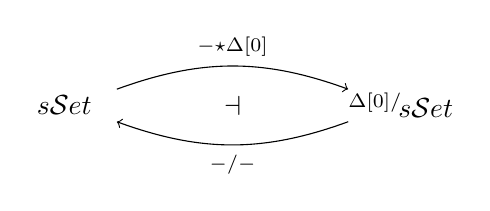
\begin{tikzpicture}[x=1.9em,y=1.4em]
  \node (s) at (0,0)   {$\sSet$};
  \node (j) at (6.4,0) {${}^{\Delta[0]/}\!\sSet$};
  \draw[->] (1.0,0.42) to[bend left=20] node[above]{$\scriptstyle-\star\Delta[0]$} (5.4,0.42);
  \node at (3.2,0) {$\dashv$};
  \draw[->] (5.4,-0.42) to[bend left=20] node[below]{$\scriptstyle-/-$} (1.0,-0.42);
\end{tikzpicture}
\end{center}
\trSphere{} $u\colon\partial\Delta[n]\to A_{/t}$ 经转置成为带末顶点 $t$ 的映射
$\Lambda^{n+1}[n+1]\to A$，而单纯形 $v\colon\Delta[n]\to A$ 则为该%
\trHorn{}的开口面提供一个填充体。于是，该\trLifting{}问题经转置便定义了
一个带末顶点 $t$ 的\trSphere{} $\partial\Delta[n+1]\to A$；所求的提升
$w\colon\Delta[n]\to A_{/t}$ 恰在这个经转置的\trSphere{}容许一个填充体时存在。
如此，我们便看到，右提升性质
\begin{center}
\begin{tikzpicture}[x=1.5em,y=1.5em]
  \node (fa) at (-2.4,0)  {$\forall n\ge 0$};
  \node (pd) at (0.4,1.3)  {$\partial\Delta[n]$};
  \node (at) at (4.8,1.3)  {$A_{/t}$};
  \node (dn) at (0.4,-1.5) {$\Delta[n]$};
  \node (a)  at (4.8,-1.5) {$A$};
  \draw[->] (1.4,1.3) -- node[above]{$\scriptstyle u$} (3.7,1.3);
  \draw[right hook->] (0.4,0.9) -- (0.4,-1.1);
  \draw[->] (1.4,-1.5) -- node[below]{$\scriptstyle v$} (3.7,-1.5);
  \draw[->] (4.8,0.9) -- (4.8,-1.1);
  \draw[->,dashed] (0.9,-1.25) -- (4.0,1.0);
  \node at (2.1,-0.1) {$\scriptstyle w$};
  \node at (7.4,0) {$\;\leftrightsquigarrow\;$};
  \begin{scope}[shift={(8.8,0)}]
  \node (o)   at (0,1.3)    {$1$};
  \node (pd2) at (3.4,1.3)  {$\partial\Delta[n]$};
  \node (a2)  at (7.4,1.3)  {$A$};
  \node (dn2) at (3.4,-1.5) {$\Delta[n]$};
  \draw[->] (o) -- node[below,pos=0.6]{$\scriptstyle\{n\}$} (pd2);
  \draw[->] (pd2) -- (a2);
  \draw[->] (o) to[bend left=25] node[above,pos=0.5]{$\scriptstyle t$} (a2);
  \draw[right hook->] (3.4,0.9) -- (3.4,-1.1);
  \draw[->,dashed] (3.75,-1.25) -- (7.0,1.0);
  \end{scope}
  \node (fa2) at (18.4,0) {$\forall n\ge 1$};
\end{tikzpicture}
\end{center}
互为转置，这就证明了 (v) 与 (vi) 的等价性。
\end{proof}

Joyal 的刻画 (vi) 有如下一个相对化的扩充：

\begin{lemma}\label{lem:relative-terminal-element-lifting}
设 $E$ 与 $B$ 是容有\trTerminal{}\trElement{}的\trQuasiCategory，且
$p\colon E\twoheadrightarrow B$ 是保持它们的\trIsofibration——意即：若 $t$
是 $E$ 的\trTerminal{}\trElement，则 $pt$ 是 $B$ 的\trTerminal{}\trElement{}。
那么任何如下形式的\trLifting{}问题都有解
\begin{center}
\begin{tikzpicture}[x=1.9em,y=1.4em]
  \node (o)  at (0,1.3)    {$1$};
  \node (pd) at (3.4,1.3)  {$\partial\Delta[n]$};
  \node (e)  at (7.6,1.3)  {$E$};
  \node (dn) at (3.4,-1.5) {$\Delta[n]$};
  \node (b)  at (7.6,-1.5) {$B$};
  \draw[->] (o) -- node[below]{$\scriptstyle\{n\}$} (pd);
  \draw[->] (pd) -- node[above]{$\scriptstyle u$} (e);
  \draw[->] (o) to[bend left=25] node[above,pos=0.5]{$\scriptstyle t$} (e);
  \draw[right hook->] (3.4,0.95) -- (3.4,-1.15);
  \draw[->,dashed] (3.75,-1.3) -- (7.2,1.0);
  \draw[->] (7.6,0.95) -- node[right]{$\scriptstyle p$} (7.6,-1.15);
  \draw[->] (dn) -- node[below]{$\scriptstyle v$} (b);
\end{tikzpicture}
\end{center}
\end{lemma}

\begin{proof}
利用 $E$ 中\trTerminal{}\trElement{} $t$ 的\trUniversalProperty{}以及%
\cref{prop:terminal-element-equivalences}(vi)，我们可以把\trSphere{} $u$ 扩充为
一个映射 $w\colon\Delta[n]\to E$。这就定义了两个映射
$pw\colon\Delta[n]\to B$ 与 $v\colon\Delta[n]\to B$，它们拥有公共边界
$pu\colon\partial\Delta[n]\to B$；由此可以定义一个\trSphere
$h\colon\partial\Delta[n+1]\to B$，使之满足 $h\delta^{n+1}=pw$ 与
$h\delta^{n}=v$——做法是：从退化\trSimplex{}
$pw\sigma^{n}\colon\Delta[n+1]\to B$ 出发，将其限制到边界上，再把该\trSphere{}中的
第 $n$ 个面替换为 $v\colon\Delta[n]\to B$。由构造，$h$ 把顶点 $\{n+1\}$ 送到 $pt$，而后者是
$B$ 的\trTerminal{}\trElement；于是我们便可以填充这个\trSphere，定义出一个单纯形
$k\colon\Delta[n+1]\to B$。

我们通过限制退化\trSimplex{} $w\sigma^{n}\colon\Delta[n+1]\to E$ 来构造
一个\trHorn{} $g\colon\Lambda^{n}[n+1]\to E$。这一对映射定义出陈述中那个
交换方块的因子分解：
\begin{center}
\begin{tikzpicture}[x=1.9em,y=1.5em]
  \node (pd) at (0,1.3)    {$\partial\Delta[n]$};
  \node (e)  at (3.2,1.3)  {$E$};
  \node (dn) at (0,-1.5)   {$\Delta[n]$};
  \node (b)  at (3.2,-1.5) {$B$};
  \draw[->] (1.0,1.3) -- node[above]{$\scriptstyle u$} (2.1,1.3);
  \draw[right hook->] (0,0.9) -- (0,-1.1);
  \draw[->] (1.0,-1.5) -- node[below]{$\scriptstyle v$} (2.1,-1.5);
  \draw[->] (3.2,0.9) -- node[right]{$\scriptstyle p$} (3.2,-1.1);
  \node at (4.7,0) {$=$};
  \begin{scope}[shift={(6.2,0)}]
  \node (pd2) at (0,1.3)    {$\partial\Delta[n]$};
  \node (la)  at (3.8,1.3)  {$\Lambda^{n}[n+1]$};
  \node (e2)  at (8.0,1.3)  {$E$};
  \node (dn2) at (0,-1.5)   {$\Delta[n]$};
  \node (dn1) at (3.8,-1.5) {$\Delta[n+1]$};
  \node (b2)  at (8.0,-1.5) {$B$};
  \draw[->] (1.0,1.3) -- node[above]{$\scriptstyle\delta^{n}$} (2.6,1.3);
  \draw[->] (5.1,1.3) -- node[above]{$\scriptstyle g$} (6.9,1.3);
  \draw[right hook->] (0,0.9) -- (0,-1.1);
  \draw[right hook->] (3.8,0.9) -- (3.8,-1.1);
  \draw[->,dashed] (4.15,-1.3) -- (7.6,1.0);
  \node at (6.15,-0.45) {$\scriptstyle\ell$};
  \draw[->] (8.0,0.9) -- node[right]{$\scriptstyle p$} (8.0,-1.1);
  \draw[->] (1.0,-1.5) -- node[below]{$\scriptstyle\delta^{n}$} (2.6,-1.5);
  \draw[->] (5.1,-1.5) -- node[below]{$\scriptstyle k$} (6.9,-1.5);
  \end{scope}
\end{tikzpicture}
\end{center}
由于这个交换矩形的中央竖直映射是一个内\trHorn{}包含，而其右手竖直映射是
拟范畴之间的一个\trIsofibration，故右边的\trLifting{}问题如所标记的那样有解
$\ell\colon\Delta[n+1]\to E$；于是显然，映射
$\ell\delta^{n}\colon\Delta[n]\to E$ 便为原来的\trLifting{}问题提供一个解。
\end{proof}

\subsection*{练习}

\begin{exercise}\label{ex:relative-lifting-arbitrary-functor}
证明：若 $A$ 与 $B$ 是容有\trTerminal{}\trElement{}的\trQuasiCategory，且
$f\colon A\to B$ 是一个保持诸\trTerminal{}\trElement{}的\trFunctor（未必是%
\trIsofibration），那么给定任何如下左图所示、其中 $t$ 是 $A$ 的%
\trTerminal{}\trElement{}的\trLifting{}问题
\begin{center}
\begin{tikzpicture}[x=1.9em,y=1.4em]
  \node (o)  at (0,1.3)    {$1$};
  \node (pd) at (3.4,1.3)  {$\partial\Delta[n]$};
  \node (a)  at (7.6,1.3)  {$A$};
  \node (dn) at (3.4,-1.5) {$\Delta[n]$};
  \node (b)  at (7.6,-1.5) {$B$};
  \draw[->] (o) -- node[below]{$\scriptstyle\{n\}$} (pd);
  \draw[->] (pd) -- (a);
  \draw[->] (o) to[bend left=25] node[above,pos=0.5]{$\scriptstyle t$} (a);
  \draw[right hook->] (3.4,0.95) -- (3.4,-1.15);
  \draw[->] (dn) -- (b);
  \draw[->] (7.6,0.95) -- node[right]{$\scriptstyle f$} (7.6,-1.15);
  \node at (9.8,0) {$\;\leftrightsquigarrow\;$};
  \begin{scope}[shift={(11.6,0)}]
  \node (pd2) at (0,1.3)    {$\partial\Delta[n]$};
  \node (a2)  at (4.4,1.3)  {$A$};
  \node (dn2) at (0,-1.5)   {$\Delta[n]$};
  \node (b2)  at (4.4,-1.5) {$B$};
  \draw[->] (1.0,1.3) -- (3.3,1.3);
  \draw[right hook->] (0,0.95) -- (0,-1.15);
  \draw[->] (1.0,-1.5) -- (3.3,-1.5);
  \draw[->] (4.4,0.95) -- node[right]{$\scriptstyle f$} (4.4,-1.15);
  \draw[->,dashed] (0.35,-1.3) -- (3.9,1.0);
  \node at (3.0,0.35) {$\scriptstyle\Downarrow\cong$};
  \end{scope}
\end{tikzpicture}
\end{center}
都存在如上右图所示的一个提升，使得左上三角在自然同构的意义下交换，而右下
三角严格交换。
\end{exercise}

\begin{exercise}\label{ex:initial-element-equivalences}
陈述并证明拟范畴中\trInitial{}\trElement{}的各种综合定义与解析定义之间的
等价。
\end{exercise}

   %

\providecommand{\Hom}{\operatorname{Hom}}
\providecommand{\rvTranspose}[1]{\ulcorner #1\urcorner}%

\section{极限与余极限}\label{sec:f-limits-and-colimits}

本节中，我们扩展\cref{prop:limits-as-terminal-cones}，证明以\trSimplicialSet{}为索引、
取值于\trQuasiCategory{}的\trDiagram{}的\trLimit{}的综合定义，与 Joyal \cite[4.5]{bib61} 最先引入的
解析定义相一致。我们证明\trLimit{}锥的四个综合定义——(i) 最初的%
\cref{def:limit-colimit-cones}；(ii) 出现于\cref{prop:absolute-right-lifting-res}中的那个；(iii) 出现于\cref{def:limit-colimit-diagrams}与\cref{prop:limit-pointwise-extension-transpose}中的那个；以及 (iv) 来自%
\cref{prop:limits-as-terminal-cones}的那个——与一个解析定义 (v)（即 Joyal
的定义）之间的等价性。此时，凭借刚才所引的诸结果以及%
\cref{prop:terminal-element-equivalences}，除了陈述该结果并为其各组成部分
提供出处之外，已无事可做。

\begin{proposition}\label{prop:limit-cone-equivalences}
考虑\trQuasiCategory{}之间的\trFunctor{} $d\colon J\to A$ 以及\trCone{} $\lambda\colon\Delta\ell\Rightarrow d$。
以下条件等价：
\begin{enumerate}[label=(\roman*)]
\item 对 $(\ell,\lambda)$ 定义一个\trAbsoluteRightLifting{}图表
\begin{center}
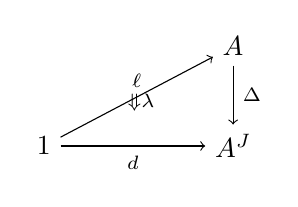
\begin{tikzpicture}[x=1.9em,y=1.5em]
  \node (a)  at (3.6,1.2)  {$A$};
  \node (aj) at (3.6,-1.2) {$A^{J}$};
  \node (o)  at (0,-1.2)   {$1$};
  \draw[->] (o) -- node[above]{$\scriptstyle\ell$} (a);
  \draw[->] (a) -- node[right]{$\scriptstyle\Delta$} (aj);
  \draw[->] (o) -- node[below]{$\scriptstyle d$} (aj);
  \node at (1.85,-0.15) {$\scriptstyle\Downarrow\lambda$};
\end{tikzpicture}
\end{center}
\item \trCone{} $\rvTranspose{\lambda}\colon 1\to A^{J\triangleleft}$ 定义一个%
\trAbsoluteRightLifting{}图表
\begin{center}
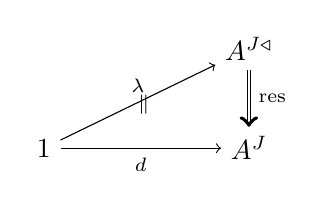
\begin{tikzpicture}[x=1.9em,y=1.5em]
  \node (ajl) at (3.9,1.2)  {$A^{J\triangleleft}$};
  \node (aj)  at (3.9,-1.2) {$A^{J}$};
  \node (o)   at (0,-1.2)   {$1$};
  \draw[->] (o) -- node[above]{$\scriptstyle\rvTranspose{\lambda}$} (ajl);
  \draw[double,->] (ajl) -- node[right]{$\scriptstyle\mathrm{res}$} (aj);
  \draw[->] (o) -- node[below]{$\scriptstyle d$} (aj);
  \node at (1.9,-0.15) {$\scriptstyle\parallel$};
\end{tikzpicture}
\end{center}
\item \trCone{} $\lambda\colon\ell!\Rightarrow d$ 定义一个逐点右扩张图表
\begin{center}
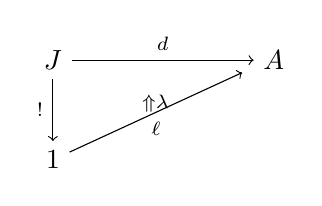
\begin{tikzpicture}[x=1.9em,y=1.5em]
  \node (j) at (0,1.2)   {$J$};
  \node (a) at (4.2,1.2) {$A$};
  \node (o) at (0,-1.2)  {$1$};
  \draw[->] (j) -- node[above]{$\scriptstyle d$} (a);
  \draw[->] (j) -- node[left]{$\scriptstyle !$} (o);
  \draw[->] (o) -- node[below,pos=0.5]{$\scriptstyle\ell$} (3.6,0.9);
  \node at (1.95,0.15) {$\scriptstyle\Uparrow\lambda$};
\end{tikzpicture}
\end{center}
\item \begingroup
\emergencystretch=3em
\trCone{}的\trQuasiCategory{} $\Hom_{A^{J}}(\Delta,d)$ 容有一个\trTerminal{}\trElement
$\rvTranspose{\lambda}\colon 1\to\Hom_{A^{J}}(\Delta,d)$，表示\trCone
$\lambda\colon\Delta\ell\Rightarrow d$。
\par\endgroup
\item \trQuasiCategory{} $A_{/d}$ 容有一个\trTerminal{}\trElement{} $\rvTranspose{\lambda}\colon 1\to A_{/d}$，
经转置定义 $d$ 到\trDiagram{} $J^{\triangleleft}\to A$ 的一个\trExtension
\begin{center}
\begin{tikzpicture}[x=1.9em,y=1.5em]
  \node (j)  at (2.2,1.4)  {$J$};
  \node (jl) at (0,-1.0)   {$J^{\triangleleft}$};
  \node (a)  at (4.6,-1.0) {$A$};
  \draw[right hook->] (j) -- (jl);
  \draw[->] (j) -- node[right,pos=0.6]{$\scriptstyle d$} (a);
  \draw[->] (jl) -- node[below]{$\scriptstyle\rvTranspose{\lambda}$} (a);
\end{tikzpicture}
\end{center}
\end{enumerate}
\end{proposition}

当这些条件成立时，以 $(\ell,\lambda)$ 或 $\rvTranspose{\lambda}$ 各种方式标记的
数据，定义了 $d$ 上的\textbf{\trLimit{}锥}。

注意，任何以\trSimplicialSet{}为索引、取值于\trQuasiCategory{}的\trDiagram{} $d'\colon J'\to A$，都可以沿一个
内\trAnodyneExtension，扩充为\trQuasiCategory{}之间的一个\trWeakEquivalence{}\trDiagram{} $d\colon J\to A$。或者在
(i)、(ii)、(iv)、(v) 诸情形中直接处理原始\trDiagram{}亦无任何代价，因为\trDiagram{}的\trQuasiCategory
$A^{J}\simeq A^{J'}$、\trCone{}的\trQuasiCategory{} $\Hom_{A^{J}}(\Delta,d)\simeq\Hom_{A^{J'}}(\Delta,d')$ 以及 $A_{/d}\simeq A_{/d'}$ 都是等价的。

\begin{proof}
(i) 与 (ii) 的等价性由\cref{prop:absolute-right-lifting-res}对任何%
\trInfinityCategory{} $A$ 与\trSimplicialSet{} $J$ 证明；而%
\trSimplicialSet{} $J^{\triangleleft}\coloneqq 1\star J$ 是\cref{def:join}中的\trJoin。(i) 与 (iii)
的等价性由\cref{prop:limit-pointwise-extension-transpose}对任何%
\trCartesianClosed{}\trInfinityCosmos{}证明。\cref{prop:limits-as-terminal-cones}证明了：对取值于任何%
\trInfinityCategory{}的任何\trDiagram{}，(i) 与 (iv) 之间的等价性都成立。

最后，(iv) 与 (v) 之间的等价性是\cref{prop:slices-cones-equivalence}所给出的、
卧于 $A$ 之上的\trQuasiCategory\trEquivalence{}
$\Hom_{A^{J}}(\Delta,d)\simeq A_{/d}$ 的一个推论；该命题给出 $d$ 之上\trCone{}的%
\trQuasiCategory{}的两个模型。最后一个要素是%
\cref{lem:equivalence-invariance-initial-elements}，它证明：这些%
\trQuasiCategory{}中若有一个容有\trTerminal{}\trElement{}，则两者皆然，因为%
\trTerminal{}\trElement{}被诸\trEquivalence{}保持。
\end{proof}

\subsection*{练习}

\begin{exercise}\label{ex:colimit-equivalences}
陈述并证明取值于\trQuasiCategory{}的\trDiagram{}的\trColimit{}的各种综合定义与解析定义之间的\trEquivalence。
\end{exercise}

   %

\section{右伴随右逆伴随}\label{sec:rajri-quasi-categories}

据我们所知，拟范畴之间的\trRightAdjoint\trRightInverse\trAdjunction{}尚未受到
多少关注。尽管如此，我们不妨驻足于此，确立这类\trAdjunction{}的一个有用的%
解析刻画，它将帮助我们比较其余各种综合定义与解析定义。

\begin{lemma}\label{lem:rajri-lifting}
拟范畴之间的\trIsofibration{} $f\colon B\twoheadrightarrow A$ 容许一个%
\trRightAdjoint\trRightInverse，当且仅当对每个\trElement{} $a\colon 1\to A$，
都存在一个满足 $fua=a$ 的\trElement{} $ua\colon 1\to B$，它具有如下性质：
任何形如下式且带 $n\ge 1$ 的\trLifting{}问题都有解
\begin{rveq}\label{eq:rajri-lifting}
\begin{tikzpicture}[x=1.9em,y=1.4em]
  \node (o)  at (0,1.4)    {$1$};
  \node (pd) at (3.4,1.4)  {$\partial\Delta[n]$};
  \node (b)  at (7.4,1.4)  {$B$};
  \node (dn) at (3.4,-1.2) {$\Delta[n]$};
  \node (a)  at (7.4,-1.2) {$A$};
  \draw[->] (o) -- node[below]{$\scriptstyle\{n\}$} (pd);
  \draw[->] (pd) -- (b);
  \draw[->] (o) to[bend left=28] node[above,pos=0.5]{$\scriptstyle ua$} (b);
  \draw[right hook->] (3.4,1.05) -- (3.4,-0.85);
  \draw[->] (b) -- node[right]{$\scriptstyle f$} (a);
  \draw[->] (dn) -- (a);
  \draw[->,dashed] (3.75,-0.95) -- (7.0,1.1);
\end{tikzpicture}
\end{rveq}
\end{lemma}

\providecommand{\rvTranspose}[1]{\ulcorner #1\urcorner}%

\begin{proof}
若 $f\colon B\twoheadrightarrow A$ 是拟范畴之间的一个\trIsofibration，容许一个%
\trRightAdjoint\trRightInverse，则由\cref{lem:rajri-fibered-adjunction}，其%
\trRightAdjoint{} $u$ 可以选取使得\trCounit{} $\epsilon\colon fu=\mathrm{id}_{A}$%
为恒等，且该\trAdjunction{}纤维化于 $A$ 之上。在此情形，%
\cref{prop:adjunction-as-fibered-equivalence}的诱导\trFiberedEquivalence{}%
$\rvTranspose{\epsilon\circ f(-)}\colon\mathrm{Hom}_{B}(B,u)\rightsquigarrow\mathrm{Hom}_{A}(f,A)$ 由\cref{prop:maps-between-commas}所定义的、$f$ 在诸%
\trCommaInfinityCategory{}之间诱导的那个映射所表示。
\begin{center}
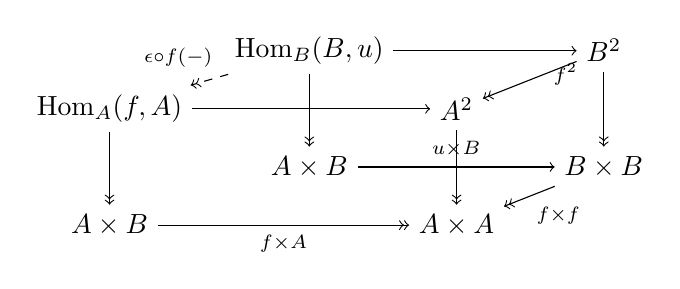
\begin{tikzpicture}[x=1.9em,y=1.5em]
  \node (hbu) at (2.2,2.8)   {$\mathrm{Hom}_{B}(B,u)$};
  \node (b2)  at (7.8,2.8)   {$B^{2}$};
  \node (hfa) at (-1.6,1.4)  {$\mathrm{Hom}_{A}(f,A)$};
  \node (a2)  at (5.0,1.4)   {$A^{2}$};
  \node (abx) at (2.2,0)     {$A\times B$};
  \node (bbx) at (7.8,0)     {$B\times B$};
  \node (bxa) at (-1.6,-1.4) {$A\times B$};
  \node (axa) at (5.0,-1.4)  {$A\times A$};
  \draw[->] (hbu) -- (b2);
  \draw[->] (hfa) -- (a2);
  \draw[->>] (b2) -- node[right,pos=0.35]{$\scriptstyle f^{2}$} (a2);
  \draw[->>] (b2) -- (bbx);
  \draw[->>] (a2) -- (axa);
  \draw[->>] (hbu) -- (abx);
  \draw[->>] (hfa) -- (bxa);
  \draw[->] (abx) -- node[above]{$\scriptstyle u\times B$} (bbx);
  \draw[->>] (bxa) -- node[below]{$\scriptstyle f\times A$} (axa);
  \draw[->>] (bbx) -- node[below right,pos=0.55]{$\scriptstyle f\times f$} (axa);
  \draw[->>,dashed] (hbu) --
    node[above,pos=0.3,xshift=-14pt]{$\scriptstyle\rvTranspose{\epsilon\circ f(-)}$} (hfa);
  \node at (2.7,2.15)  {$\scriptstyle\urcorner$};
  \node at (-1.05,0.75){$\scriptstyle\lrcorner$};
\end{tikzpicture}
\end{center}
凭借该结果——或者换个途径，凭借其证明所依赖的\cref{prop:pullback-map-fibration}%
——我们便看到，诸\trCommaInfinityCategory{}之间的诱导映射也是一个%
\trIsofibration。结合这两件事实，可知 $\rvTranspose{\epsilon\circ f(-)}\colon\mathrm{Hom}_{B}(B,u)\twoheadrightarrow\mathrm{Hom}_{A}(f,A)$ 是
$A\times B$ 之上的一个\trTrivialFibration。这一\trTrivialFibration{}沿任意%
顶点 $a\colon 1\to A$ 拉回，定义了 $B$ 之上的一个\trTrivialFibration{}%
$\mathrm{Hom}_{B}(B,ua)\twoheadrightarrow\mathrm{Hom}_{A}(f,a)$。由%
\cref{cor:slice-cone-point}，其定义域与陪域都\trEquivalence{}于 Joyal 的切片，
于是由 $f$ 诱导出的\trIsofibration{} $f\colon B_{/ua}\twoheadrightarrow f_{/a}$ 同样是拟范畴之间的一个\trTrivialFibration。\cref{def:trivial-fibration}%
的定义性\trLifting{}性质
\begin{center}
\begin{tikzpicture}[x=1.9em,y=1.4em]
  \node (pd) at (0,1.2)    {$\partial\Delta[n-1]$};
  \node (bu) at (5.2,1.2)  {$B_{/ua}$};
  \node (dn) at (0,-1.2)   {$\Delta[n-1]$};
  \node (fa) at (5.2,-1.2) {$f_{/a}$};
  \draw[->] (pd) -- (bu);
  \draw[right hook->] (0,0.85) -- (0,-0.85);
  \draw[->,dashed] (0.5,-0.85) -- (4.6,0.95);
  \draw[->] (5.2,0.85) -- (5.2,-0.85);
  \draw[->,shorten >=0.35em] (5.2,0.85) -- (5.2,-0.85);
  \node at (5.62,0) {$\scriptstyle f$};
  \draw[->] (dn) -- (fa);
\end{tikzpicture}
\end{center}
当 $n\ge 1$ 时经转置便成为 \eqref{eq:rajri-lifting} 的那个\trLifting{}性质。

反之，\eqref{eq:rajri-lifting} 的那个\trLifting{}性质可用来归纳地定义 $f$ 的%
一个\trSection{} $u\colon A\to B$，它扩充诸\trElement{} $ua\colon 1\to B$ 的%
选取——其中每个 $ua$ 提升相应的 $a\colon 1\to A$。包含 $\mathrm{sk}_{0}A\hookrightarrow A$ 可以表示为映射 $\partial\Delta[n]\hookrightarrow\Delta[n]$%
（$n\ge 1$）的\trCoproduct{}之\trPushout{}的一个可数复合，而
\begin{center}
\begin{tikzpicture}[x=1.9em,y=1.4em]
  \node (o)  at (0,1.4)    {$1$};
  \node (sk) at (3.4,1.4)  {$\mathrm{sk}_{0}A$};
  \node (b)  at (7.2,1.4)  {$B$};
  \node (a1) at (3.4,-1.2) {$A$};
  \node (a2) at (7.2,-1.2) {$A$};
  \draw[->] (o) -- node[below]{$\scriptstyle a$} (sk);
  \draw[->] (sk) -- node[below]{$\scriptstyle u$} (b);
  \draw[->] (o) to[bend left=25] node[above,pos=0.5]{$\scriptstyle ua$} (b);
  \draw[right hook->] (3.4,1.05) -- (3.4,-0.85);
  \draw[->] (b) -- node[right]{$\scriptstyle f$} (a2);
  \draw[double] (a1) -- (a2);
  \draw[->,dashed] (3.75,-0.95) -- (6.85,1.1);
\end{tikzpicture}
\end{center}
定义一个提升所需的每个中间\trLifting{}问题都具有 \eqref{eq:rajri-lifting}
之形。要证明 $u$ 是 $f$ 的一个\trRightAdjoint\trRightInverse，据%
\cref{lem:rajri-modification}，只需定义一个 2-\trCell{} $\eta\colon\mathrm{id}_{B}\Rightarrow uf$，它与 $u$ 及与 $f$ 作\trWhiskering{}后皆成为%
\trIsomorphism{}即可。我们通过求解如下\trLifting{}问题来构造 $\eta$ 的一个代表
\begin{center}
\begin{tikzpicture}[x=1.9em,y=1.4em]
  \node (bb) at (0,1.4)    {$B\sqcup B$};
  \node (b)  at (6.2,1.4)  {$B$};
  \node (bd) at (0,-1.2)   {$B\times\Delta[1]$};
  \node (b2) at (3.9,-1.2) {$B$};
  \node (a)  at (7.2,-1.2) {$A$};
  \draw[->] (bb) -- node[above]{$\scriptstyle\mathrm{id}_{B}\sqcup uf$} (b);
  \draw[right hook->] (0,1.05) -- (0,-0.85);
  \draw[->,dashed] (0.5,-0.9) -- (5.75,1.1);
  \node at (3.2,0.3) {$\scriptstyle\eta$};
  \draw[->] (6.2,1.05) -- node[right]{$\scriptstyle f$} (6.2,-0.85);
  \draw[->] (bd) -- node[below]{$\scriptstyle\pi$} (b2);
  \draw[->] (b2) -- node[below]{$\scriptstyle f$} (a);
\end{tikzpicture}
\end{center}
它同样为 \eqref{eq:rajri-lifting} 所允许；注意包含 $B\sqcup B\hookrightarrow B\times\Delta[1]$ 在顶点上是双射，并进一步注意：陪域中凡定义域所缺失的单纯形，
其末顶点都落在 $u$ 的像之中。由构造，$f\eta=\mathrm{id}_{f}$ 当然可逆。

要证明 $\eta u$ 是一个\trIsomorphism，据\cref{cor:edge-isomorphism-components}，
只需检验其诸分量 $\eta u(a)\colon ua\to ufua=ua$ 皆是 $B$ 中的%
\trIsomorphism{}即可。\footnote{原书印作「isomorphisms in $A$」，疑为
「in $B$」之误，此处径改。——译者注}这些分量的逆\trIsomorphism{}可以经由
\eqref{eq:rajri-lifting} 之\trLifting{}性质的初等运用找到，其细节留给读者。
\end{proof}

\subsection*{练习}

\begin{exercise}\label{ex:rajri-composite}
验证\cref{lem:rajri-lifting}的证明中作出的最后一论断。
\end{exercise}

\begin{exercise}\label{ex:lari-lifting-analog}
表述一个类似的\trLifting{}性质，用以刻画容许\trLeftAdjoint\trRightInverse{}的
那些\trIsofibration{} $f\colon B\twoheadrightarrow A$。
\end{exercise}

   %

\providecommand{\sSet}{s\mathcal{S}et}%
\providecommand{\qcThree}{\mathbf{3}} %
\providecommand{\rvTranspose}[1]{\ulcorner #1\urcorner}%
\providecommand{\QCat}{\mathcal{Q}\mathit{Cat}}%
\providecommand{\cellpair}[5]{$\vcenter{\hbox{\begin{tikzpicture}[x=1.15em,y=1.15em]%
\node (s) at (0,0) {$#1$};%
\node (t) at (4.2,0) {$#2$};%
\draw[->] (0.75,0.32) to[bend left=18] (3.45,0.32);%
\node at (2.1,0.88) {$\scriptstyle#3$};%
\draw[->] (0.75,-0.32) to[bend right=18] (3.45,-0.32);%
\node at (2.1,-0.93) {$\scriptstyle#4$};%
\draw[->] (1.95,0.2) to[bend right=32] (1.95,-0.2);%
\node at (2.85,0) {$\scriptstyle#5$};%
\end{tikzpicture}}}$\ignorespaces}

\section{笛卡尔与余笛卡尔纤维化}\label{sec:f-cartesian-cocartesian-fibrations}

本节的目标，是确立这样一些拟范畴之间的\trIsofibration{} $p\colon E\to B$ 的%
综合刻画与解析刻画之间的等价：它们定义\trCartesianFibration{}或%
\trCocartesianFibration。我们从考察 $p$-\trCartesianArrow{}入手，证明%
\cref{thm:pcartesian-characterizations}的三个综合定义与三个解析定义——后者
出现于 \cite[2.4.1.1, 2.4.1.4, 2.4.1.8]{bib78}——之间的等价。
随后，我们对\trCartesianFibration{}的综合刻画与解析刻画证明一个类似的比较，
并利用它来强化与\trCartesianFibration{}相关联的诸\trLifting{}性质。我们最后
证明：\trDiscreteCocartesianFibration{}与 Joyal 的\trLeftFibration{}相重合，而\trDiscreteCartesianFibration{}则与%
\trRightFibration{}相重合。

在 5.1 节中，「\trCartesianArrow」这一称谓指的是广义元素%
$\rvTranspose{\psi}\colon X\to E^{2}$，或者同样地，指它所表示的那个自然变换
\cellpair{X}{E}{e'}{e}{\psi}。在\trQuasiCategory{}的\trInfinityCosmos{}中，
一支 $X$-形箭头是\trCartesian，当且仅当它在每个\trElement{} $x\colon 1\to X$
处的诸分量 $\rvTranspose{\psi x}$ 都是\trCartesian{}（见%
\cref{prop:fiberwise-equivalence-cartesian-functor}）；于是，为简化下文的
讨论，我们只考虑形如 $\rvTranspose{\psi}\colon 1\to E^{2}$ 的箭头——亦即 $E$
中的 1-\trSimplex——并以简化记号 $\psi\colon e'\to e$ 来刻画它们。

\begin{proposition}\label{prop:cartesian-arrow-analytic}
固定拟范畴之间的一条\trIsofibration{} $p\colon E\twoheadrightarrow B$。以下诸条件等价，并且
刻画了 $E$ 中的 1-\trSimplex{} $\psi\colon e'\to e$ 何时是%
\textbf{$p$-\trCartesian}：
\begin{enumerate}[label=(\roman*)]
\item 由像为 $\qcThree$ 中\trCospan{} $0\to 2\leftarrow 1$ 的那个包含
$\delta\colon\llcorner\hookrightarrow\qcThree$ 所诱导的\trIsofibration
\begin{center}
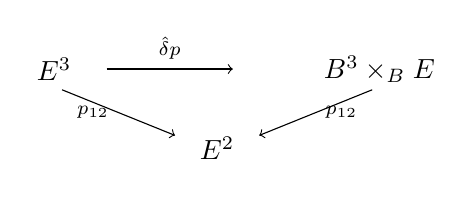
\begin{tikzpicture}[x=1.9em,y=1.5em]
  \node (E3) at (0,0)      {$E^{3}$};
  \node (Bp) at (6.2,0)    {$B^{3}\times_{B^{\llcorner}}E^{\llcorner}$};
  \node (E2) at (3.1,-1.9) {$E^{2}$};
  \draw[->] (1.0,0) -- node[above]{$\scriptstyle\hat{\delta}p$} (3.4,0);
  \draw[->] (0.15,-0.5) -- node[left]{$\scriptstyle p_{12}$} (2.3,-1.6);
  \draw[->] (6.05,-0.5) -- node[right]{$\scriptstyle p_{12}$} (3.9,-1.6);
\end{tikzpicture}
\end{center}
经拉回便在 $\psi$ 之上的\trFiber{}上定义一条\trTrivialFibration。
\item 如下左图的交换三角形定义了一个\trAbsoluteRightLifting{}图表
\begin{center}
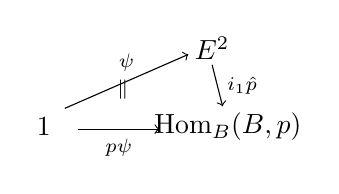
\begin{tikzpicture}[x=1.9em,y=1.5em]
  \node (o)  at (0,0)     {$1$};
  \node (E2) at (3.2,1.9) {$E^{2}$};
  \node (H)  at (3.5,0)   {$\mathrm{Hom}_{B}(B,p)$};
  \draw[->] (0.4,0.45) -- node[above,pos=0.5]{$\scriptstyle\psi$} (2.75,1.75);
  \node at (1.5,0.9) {$\scriptstyle\parallel$};
  \draw[->] (0.65,-0.05) -- node[below]{$\scriptstyle p\psi$} (2.2,-0.05);
  \draw[->] (3.2,1.5) -- node[right]{$\scriptstyle i_{1}\hat{p}$} (3.4,0.5);
\end{tikzpicture}
\quad 其中\quad
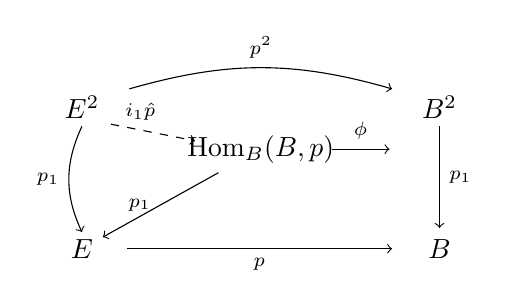
\begin{tikzpicture}[x=1.9em,y=1.5em]
  \node (E2) at (0,1.9)   {$E^{2}$};
  \node (B2) at (6.8,1.9) {$B^{2}$};
  \node (H)  at (3.4,0.9) {$\mathrm{Hom}_{B}(B,p)$};
  \node (E)  at (0,-1.5)  {$E$};
  \node (B)  at (6.8,-1.5){$B$};
  \draw[->] (0.9,2.35) to[bend left=16] node[above]{$\scriptstyle p^{2}$} (5.9,2.35);
  \draw[->,dashed] (0.55,1.5) -- node[above,pos=0.35]{$\scriptstyle i_{1}\hat{p}$} (2.15,1.1);
  \draw[->] (4.75,0.9) -- node[above]{$\scriptstyle\rvTranspose{\phi}$} (5.85,0.9);
  \draw[->] (0,1.45) to[bend right=25] node[left,pos=0.5]{$\scriptstyle p_{1}$} (0,-1.1);
  \draw[->] (H) -- node[left]{$\scriptstyle p_{1}$} (E);
  \draw[->] (6.8,1.45) -- node[right]{$\scriptstyle p_{1}$} (6.8,-1.0);
  \draw[->] (0.85,-1.5) -- node[below]{$\scriptstyle p$} (5.9,-1.5);
  \node at (3.9,0.5) {$\scriptstyle\llcorner$};
\end{tikzpicture}
\end{center}
\item 存在一个\trAbsoluteRightLifting{}图表，满足 $p_{1}\epsilon=\psi$ 与
$p_{0}\epsilon=\mathrm{id}_{pe'}$：
\begin{center}
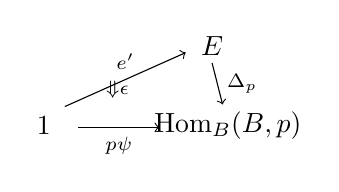
\begin{tikzpicture}[x=1.9em,y=1.5em]
  \node (o)  at (0,0)   {$1$};
  \node (E)  at (3.2,1.9) {$E$};
  \node (H)  at (3.5,0) {$\mathrm{Hom}_{B}(B,p)$};
  \draw[->] (0.4,0.45) -- node[above,pos=0.5]{$\scriptstyle e'$} (2.7,1.75);
  \node at (1.4,0.85) {$\scriptstyle\Downarrow\epsilon$};
  \draw[->] (0.65,-0.05) -- node[below]{$\scriptstyle p\psi$} (2.2,-0.05);
  \draw[->] (3.2,1.5) -- node[right]{$\scriptstyle\Delta_{p}$} (3.4,0.5);
\end{tikzpicture}
\quad 其中\quad
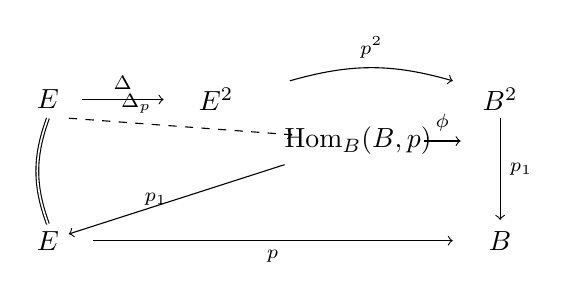
\begin{tikzpicture}[x=1.9em,y=1.5em]
  \node (E1) at (0,1.9)   {$E$};
  \node (E2) at (3.2,1.9) {$E^{2}$};
  \node (B2) at (8.6,1.9) {$B^{2}$};
  \node (H)  at (5.9,0.9) {$\mathrm{Hom}_{B}(B,p)$};
  \node (Eb) at (0,-1.5)  {$E$};
  \node (B)  at (8.6,-1.5){$B$};
  \draw[->] (0.65,1.9) -- node[above]{$\scriptstyle\Delta$} (2.2,1.9);
  \draw[->] (4.6,2.35) to[bend left=16] node[above]{$\scriptstyle p^{2}$} (7.7,2.35);
  \draw[->,dashed] (0.4,1.45) -- node[above,pos=0.3]{$\scriptstyle\Delta_{p}$} (4.65,1.05);
  \draw[->] (7.15,0.9) -- node[above]{$\scriptstyle\rvTranspose{\phi}$} (7.85,0.9);
  \draw[double] (0,1.45) to[bend right=20] (0,-1.1);
  \draw[->] (H) -- node[left]{$\scriptstyle p_{1}$} (Eb);
  \draw[->] (8.6,1.45) -- node[right]{$\scriptstyle p_{1}$} (8.6,-1.0);
  \draw[->] (0.85,-1.5) -- node[below]{$\scriptstyle p$} (7.7,-1.5);
  \node at (6.35,0.5) {$\scriptstyle\llcorner$};
\end{tikzpicture}
\end{center}
\item 方块
\begin{center}
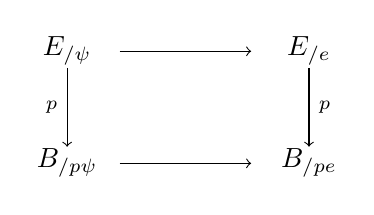
\begin{tikzpicture}[x=1.9em,y=1.5em]
  \node (Ep) at (0,1.3)   {$E_{/\psi}$};
  \node (Ee) at (4.6,1.3) {$E_{/e}$};
  \node (Bp) at (0,-1.4)  {$B_{/p\psi}$};
  \node (Be) at (4.6,-1.4){$B_{/pe}$};
  \draw[->] (1.0,1.3) -- (3.5,1.3);
  \draw[->] (0,0.9) -- node[left]{$\scriptstyle p$} (0,-1.0);
  \draw[->] (4.6,0.9) -- node[right]{$\scriptstyle p$} (4.6,-1.0);
  \draw[->] (1.0,-1.4) -- (3.5,-1.4);
\end{tikzpicture}
\end{center}
中到拉回的诱导映射是一条\trTrivialFibration{}
$E_{/\psi}\twoheadrightarrow B_{/p\psi}\mathbin{\underset{B_{/pe}}{\times}}E_{/e}$。
\item 任何 $n\ge 2$ 的如下形式的\trLifting{}问题都有解：
\begin{rveq}\label{eq:pcartesian-horn-lifting}
\begin{tikzpicture}[x=1.9em,y=1.4em]
  \node (d1) at (0,1.3)    {$\Delta[1]$};
  \node (ho) at (3.6,1.3)  {$\Lambda^{n}[n]$};
  \node (E)  at (7.4,1.3)  {$E$};
  \node (dn) at (3.6,-1.4) {$\Delta[n]$};
  \node (B)  at (7.4,-1.4) {$B$};
  \draw[->] (1.0,1.3) -- node[below]{$\scriptstyle\{n-1,n\}$} (2.6,1.3);
  \draw[->] (4.6,1.3) -- (6.4,1.3);
  \draw[->] (0.6,1.8) to[bend left=20] node[above,pos=0.5]{$\scriptstyle\psi$} (6.8,1.8);
  \draw[right hook->] (3.6,0.95) -- (3.6,-0.9);
  \draw[->,dashed] (4.0,-1.2) -- (6.9,1.0);
  \draw[->] (7.4,0.95) -- node[right]{$\scriptstyle p$} (7.4,-0.9);
  \draw[->] (4.6,-1.4) -- (6.4,-1.4);
\end{tikzpicture}
\end{rveq}
\item 任何 $n\ge 1$ 的如下形式的\trLifting{}问题都有解：
\begin{rveq}\label{eq:pcartesian-cylinder-lifting}
\begin{tikzpicture}[x=1.9em,y=1.4em]
  \node (d1)  at (0,1.3)    {$\Delta[1]$};
  \node (pd)  at (3.9,1.3)  {$\partial\Delta[n]\times\Delta[1]$};
  \node (d11) at (8.1,1.3)  {$\Delta[n]\times\{1\}$};
  \node (E)   at (10.9,1.3) {$E$};
  \node (dn)  at (5.0,-1.4) {$\Delta[n]\times\Delta[1]$};
  \node (B)   at (10.9,-1.4){$B$};
  \draw[->] (0.9,1.3) -- node[below]{$\scriptstyle\{n\}\times\mathrm{id}$} (2.3,1.3);
  \draw[->] (6.1,1.3) -- (6.9,1.3);
  \draw[->] (9.4,1.3) -- (10.2,1.3);
  \node at (6.0,1.8) {$\scriptstyle\sqcup$};
  \node at (6.0,0.7) {$\scriptstyle\partial\Delta[n]\times\{1\}$};
  \draw[->] (1.0,1.9) to[bend left=18] node[above,pos=0.45]{$\scriptstyle\psi$} (10.3,1.9);
  \draw[right hook->] (5.0,0.95) -- (5.0,-0.9);
  \draw[->,dashed] (5.5,-1.2) -- (10.4,1.0);
  \draw[->] (10.9,0.95) -- node[right]{$\scriptstyle p$} (10.9,-0.9);
  \draw[->] (6.8,-1.4) -- (9.9,-1.4);
\end{tikzpicture}
\end{rveq}
\end{enumerate}
\end{proposition}

\begin{proof}
\cref{thm:pcartesian-characterizations}在任何\trInfinityCosmos{}中证明了条件
(i)、(ii) 与 (iii) 的等价性。

由\cref{lem:dashed-square-hypercube}，(i) 中的映射同构于如下方块中到拉回的
诱导映射——该方块与 (iv) 中出现的方块十分相似。\footnote{诚然，方块
\eqref{eq:hypercube-weakly-cartesian} 中的始对象是一个我们记作 $E_{/\psi}$ 的
拟范畴，因为它\trEquivalence{}（尽管不同构）于 Joyal 的切片拟范畴（见
\cref{war:slice-notation}）。为免此处混淆，我们以 $E_{//\psi}$ 记该拟范畴，
而把记号 $E_{/\psi}$ 留给\cref{def:join}的切片拟范畴。}我们将通过在每一个%
\trWeaklyCartesianSquare{}中构造其顶行映射之间的、如下左侧所示的自然等价，来
证明这两个方块等价：
\begin{center}
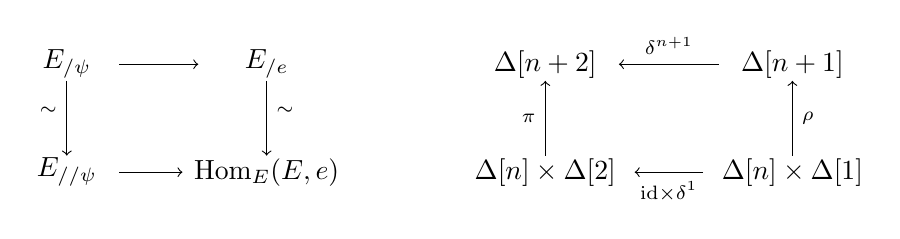
\begin{tikzpicture}[x=1.9em,y=1.5em]
  \node (l1) at (0,1.3)    {$E_{/\psi}$};
  \node (l2) at (3.8,1.3)  {$E_{/e}$};
  \node (l3) at (0,-1.3)   {$E_{//\psi}$};
  \node (l4) at (3.8,-1.3) {$\mathrm{Hom}_{E}(E,e)$};
  \draw[->] (1.0,1.3) -- (2.5,1.3);
  \draw[->] (0,0.9) -- node[left,pos=0.4]{$\scriptstyle\sim$} (0,-0.9);
  \draw[->] (3.8,0.9) -- node[right,pos=0.4]{$\scriptstyle\sim$} (3.8,-0.9);
  \draw[->] (1.0,-1.3) -- (2.2,-1.3);
  \node at (5.5,0) {$\;\leftrightsquigarrow\;$};
  \begin{scope}[shift={(7.2,0)}]
    \node (r1) at (1.9,1.3)  {$\Delta[n+2]$};
    \node (r2) at (6.6,1.3)  {$\Delta[n+1]$};
    \node (r3) at (1.9,-1.3) {$\Delta[n]\times\Delta[2]$};
    \node (r4) at (6.6,-1.3) {$\Delta[n]\times\Delta[1]$};
    \draw[->] (5.2,1.3) -- node[above]{$\scriptstyle\delta^{n+1}$} (3.3,1.3);
    \draw[->] (1.9,-0.9) -- node[left]{$\scriptstyle\pi$} (1.9,0.9);
    \draw[->] (6.6,-0.9) -- node[right]{$\scriptstyle\rho$} (6.6,0.9);
    \draw[->] (4.9,-1.3) -- node[below]{$\scriptstyle\mathrm{id}\times\delta^{1}$} (3.6,-1.3);
  \end{scope}
\end{tikzpicture}
\end{center}
此图中的诸映射，最容易借助它们在 $n$-\trSimplex{}上的作用来描述：每个映射都
沿上方右侧所示交换方块中相应的函子作限制而给出，其中 $\pi$ 与 $\rho$ 均由
如下公式定义：
\[
\rho(i,j)\coloneqq\pi(i,j)\coloneqq
\begin{cases}
i & j=0\\
n+j & j>0
\end{cases}
\]
\cref{prop:fat-join-comparison-weak-equivalence}与%
\cref{prop:slices-cones-equivalence}证明左手竖直映射是一个\trEquivalence，而
\cref{cor:slice-cone-point}则证明右手竖直映射是一个\trEquivalence。于是，这
两个方块等价，从而由\cref{lem:dashed-square-hypercube}，(i) 等价于 (iv)。

由\cref{prop:join-slice-adjunction}之\trAdjunction，刻画 (iv) 之%
\trTrivialFibration{}的那个\trLifting{}性质经转置便成为 (v) 的\trLifting{}%
性质
\begin{center}
\begin{tikzpicture}[x=1.9em,y=1.5em]
  \node (a) at (0,1.3)    {$\partial\Delta[n]$};
  \node (b) at (3.8,1.3)  {$E_{/\psi}$};
  \node (c) at (0,-1.4)   {$\Delta[n]$};
  \node (d) at (4.6,-1.4) {$B_{/p\psi}\mathbin{\underset{B_{/pe}}{\times}}E_{/e}$};
  \draw[->] (1.0,1.3) -- (2.7,1.3);
  \draw[right hook->] (0,0.9) -- (0,-1.0);
  \draw[->,dashed] (0.5,-1.2) -- (3.2,1.05);
  \draw[->] (1.0,-1.4) -- (2.9,-1.4);
  \node at (6.3,0) {$\;\leftrightsquigarrow\;$};
  \begin{scope}[shift={(8.0,0)}]
    \node (e1) at (0,1.3)    {$\Delta[1]$};
    \node (e2) at (3.8,1.3)  {$\Lambda^{n+2}[n+2]$};
    \node (e3) at (7.4,1.3)  {$E$};
    \node (e4) at (3.8,-1.4) {$\Delta[n+2]$};
    \node (e5) at (7.4,-1.4) {$B$};
    \draw[->] (0.9,1.3) -- node[below]{$\scriptstyle\{n+1,n+2\}$} (2.4,1.3);
    \draw[->] (5.4,1.3) -- (6.4,1.3);
    \draw[->] (0.6,1.8) to[bend left=20] node[above,pos=0.5]{$\scriptstyle\psi$} (6.8,1.8);
    \draw[right hook->] (3.8,0.95) -- (3.8,-0.9);
    \draw[->,dashed] (4.2,-1.2) -- (6.9,1.0);
    \draw[->] (7.4,0.95) -- node[left]{$\scriptstyle p$} (7.4,-0.9);
    \draw[->] (5.4,-1.4) -- (6.4,-1.4);
    \node at (8.9,-0.2) {对 $n\ge 0$};
  \end{scope}
\end{tikzpicture}
\end{center}
这就证明了 (iv) 等价于 (v)。

现在我们来论证 (F.4.2) 与 (F.4.3) 这两个\trLifting{}性质的等价性。其中一个
蕴含关系依据收缩图 (F.4.4) 成立
\begin{rveq}\label{eq:horn-inclusion-retract}
\begin{tikzpicture}[x=1.9em,y=1.5em]
  \node (a) at (0,1.3)     {$\Delta[1]$};
  \node (b) at (3.2,1.3)   {$\Lambda^{n+1}[n+1]$};
  \node (c) at (7.6,1.3)   {$\partial\Delta[n]\times\Delta[1]$};
  \node (d) at (11.2,1.3)  {$\Delta[n]\times\{1\}$};
  \node (e) at (14.2,1.3)  {$\Lambda^{n+1}[n+1]$};
  \node (f) at (3.2,-1.6)  {$\Delta[n+1]$};
  \node (g) at (7.6,-1.6)  {$\Delta[n]\times\Delta[1]$};
  \node (h) at (14.2,-1.6) {$\Delta[n+1]$};
  \draw[->] (a) -- node[below]{$\scriptstyle\{n,n+1\}$} (b);
  \draw[right hook->] (b) -- (c);
  \node at (9.4,1.8) {$\scriptstyle\sqcup$};
  \node at (9.4,0.7) {$\scriptstyle\partial\Delta[n]\times\{1\}$};
  \draw[->] (11.9,1.3) -- (13.1,1.3);
  \draw[->] (0.6,2.0) to[bend left=14] node[above,pos=0.35]{$\scriptstyle\{n\}\times\mathrm{id}$} (14.2,2.0);
  \draw[right hook->] (b) -- (f);
  \draw[right hook->] (9.4,0.3) -- (9.4,-1.1);
  \draw[right hook->] (e) -- (h);
  \draw[->] (6.4,-1.6) -- node[above]{$\scriptstyle\iota$} (4.5,-1.6);
  \draw[->] (8.9,-1.6) -- node[above]{$\scriptstyle\rho$} (13.1,-1.6);
\end{tikzpicture}
\end{rveq}
其中 $\rho$ 是上文定义的映射，而 $\iota$ 是它的唯一截面。由
\cref{lem:right-lifting-closure}，现在已显然：(F.4.3) 的\trLifting{}性质蕴含
(F.4.2) 的\trLifting{}性质。

反之，我们证明 (v) 中假设的\trLifting{}性质足以求解 (vi) 所提出的那一%
\trLifting{}问题。我们的任务，是为 $\Delta[n]\times\Delta[1]$ 的那 $n+1$ 个
洗牌逐个找出沿 $p$ 的提升。我们从柱面的闭端起把这些洗牌编号为
$0,\dotsc,n$。对 $k<n$ 归纳地前进，我们通过填充一个
$\Lambda^{k+1}[n+1]$-\trHorn{}来为第 $k$ 个洗牌选取一个提升；由于 $p$ 是拟
范畴之间的\trIsofibration，这是可以做到的。要提升第 $n$ 个洗牌，我们须填充
一个 $\Lambda^{n+1}[n+1]$-\trHorn{}，其最末 $\{n,n+1\}$ 边是 $\psi$；这可以
借 (F.4.2) 的\trLifting{}性质做到。这就证明了 (v)$\Longleftrightarrow$(vi)。
\end{proof}

我们的下一个结果，把\cref{thm:internal-characterization}中证明了等价性的三个
综合定义与\cref{prop:external-characterization}的第四个综合定义，同 Lurie 的
两个解析定义 \cite[\S 2.4.1--2]{bib78} 加以比较。

\begin{proposition}\label{prop:cartesian-fibration-analytic}
对拟范畴之间的一条\trIsofibration{} $p\colon E\twoheadrightarrow B$，以下诸
条件等价，并且定义了 $p$ 成为一条\textbf{\trCartesianFibration}的含义：
\begin{enumerate}[label=(\roman*)]
\item 如下左图所示的每个自然变换 $\beta\colon b\Rightarrow pe$ 都容有一个如下
右图所示的提升 $\chi\colon e'\Rightarrow e$：
\begin{center}
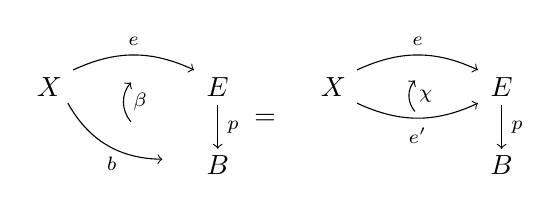
\begin{tikzpicture}[x=1.9em,y=1.5em]
  \node (X) at (0,0)     {$X$};
  \node (E) at (3.2,0)   {$E$};
  \node (B) at (3.2,-1.9){$B$};
  \draw[->] (0.45,0.4) to[bend left=25] node[above,pos=0.5]{$\scriptstyle e$} (2.75,0.4);
  \draw[->] (0.35,-0.4) to[bend right=30] node[below,pos=0.55]{$\scriptstyle b$} (2.15,-1.75);
  \draw[->] (3.2,-0.45) -- node[right]{$\scriptstyle p$} (3.2,-1.5);
  \draw[->] (1.55,-0.85) to[bend left=40] node[right]{$\scriptstyle\beta$} (1.55,0.1);
  \node at (4.1,-0.8) {$=$};
  \begin{scope}[shift={(5.4,0)}]
    \node (X2) at (0,0)     {$X$};
    \node (E2) at (3.2,0)   {$E$};
    \node (B2) at (3.2,-1.9){$B$};
    \draw[->] (0.45,0.4) to[bend left=25] node[above,pos=0.5]{$\scriptstyle e$} (2.75,0.4);
    \draw[->] (0.45,-0.4) to[bend right=25] node[below,pos=0.5]{$\scriptstyle e'$} (2.75,-0.4);
    \draw[->] (3.2,-0.45) -- node[right]{$\scriptstyle p$} (3.2,-1.5);
    \draw[->] (1.55,-0.6) to[bend left=40] node[right]{$\scriptstyle\chi$} (1.55,0.15);
  \end{scope}
\end{tikzpicture}
\end{center}
并带有如下性质：
\begin{itemize}
\item \textbf{归纳}：给定任何\trFunctor{} $f\colon Y\to X$ 与自然变换
\scalebox{0.85}{\cellpair{Y}{E}{e''}{ef}{\tau}} 和 \scalebox{0.85}{\cellpair{Y}{B}{pe''}{pe'f}{\gamma}}，满足
$p\tau=p\chi f\cdot\gamma$，则存在 $\gamma$ 的一个提升
\scalebox{0.85}{\cellpair{Y}{E}{e''}{e'f}{\bar\gamma}}，使得 $\tau=\chi f\cdot\bar\gamma$。
\item \textbf{保守性}：$\chi$ 之任何限制的纤维化自同态皆可逆：若
\cellpair{Y}{E}{e'f}{e'f}{\zeta} 是任一自然变换，满足 $\chi f\cdot\zeta=\chi f$
且 $p\zeta=\mathrm{id}_{pe'f}$，则 $\zeta$ 可逆。
\end{itemize}
\item 如下左图所示的每个自然变换 $\beta\colon b\Rightarrow pe$ 都容有一个如下
右图所示的提升 $\chi\colon e'\Rightarrow e$：
\begin{center}
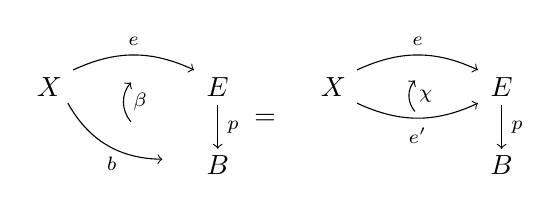
\begin{tikzpicture}[x=1.9em,y=1.5em]
  \node (X) at (0,0)     {$X$};
  \node (E) at (3.2,0)   {$E$};
  \node (B) at (3.2,-1.9){$B$};
  \draw[->] (0.45,0.4) to[bend left=25] node[above,pos=0.5]{$\scriptstyle e$} (2.75,0.4);
  \draw[->] (0.35,-0.4) to[bend right=30] node[below,pos=0.55]{$\scriptstyle b$} (2.15,-1.75);
  \draw[->] (3.2,-0.45) -- node[right]{$\scriptstyle p$} (3.2,-1.5);
  \draw[->] (1.55,-0.85) to[bend left=40] node[right]{$\scriptstyle\beta$} (1.55,0.1);
  \node at (4.1,-0.8) {$=$};
  \begin{scope}[shift={(5.4,0)}]
    \node (X2) at (0,0)     {$X$};
    \node (E2) at (3.2,0)   {$E$};
    \node (B2) at (3.2,-1.9){$B$};
    \draw[->] (0.45,0.4) to[bend left=25] node[above,pos=0.5]{$\scriptstyle e$} (2.75,0.4);
    \draw[->] (0.45,-0.4) to[bend right=25] node[below,pos=0.5]{$\scriptstyle e'$} (2.75,-0.4);
    \draw[->] (3.2,-0.45) -- node[right]{$\scriptstyle p$} (3.2,-1.5);
    \draw[->] (1.55,-0.6) to[bend left=40] node[right]{$\scriptstyle\chi$} (1.55,0.15);
  \end{scope}
\end{tikzpicture}
\end{center}
并带有如下性质：诱导映射是一条\trTrivialFibration{}
\[
E_{/\chi}\twoheadrightarrow B_{/\beta}\mathbin{\underset{B_{/pe}}{\times}}E_{/e}\text{。}
\]
\item 函子 $\Delta_{p}\colon E\to\mathrm{Hom}_{B}(B,p)$ 容有一个 $B$ 上的%
\trRightAdjoint。
\item 函子 $i_{1}\hat{p}\colon E^{2}\twoheadrightarrow\mathrm{Hom}_{B}(B,p)$
容有一个\trRightAdjoint\trRightInverse。
\item $B$ 中任何 1-\trSimplex{} $\beta\colon b\to pe$ 都容有 $E$ 中的一个提升
$\chi\colon e'\to e$，使得任何 $n\ge 1$ 的\trLifting{}问题
\begin{center}
\begin{tikzpicture}[x=1.9em,y=1.4em]
  \node (d1)  at (0,1.3)    {$\Delta[1]$};
  \node (pd)  at (3.9,1.3)  {$\partial\Delta[n]\times\Delta[1]$};
  \node (d11) at (8.1,1.3)  {$\Delta[n]\times\{1\}$};
  \node (E)   at (10.9,1.3) {$E$};
  \node (dn)  at (5.0,-1.4) {$\Delta[n]\times\Delta[1]$};
  \node (B)   at (10.9,-1.4){$B$};
  \draw[->] (0.9,1.3) -- node[below]{$\scriptstyle\{n\}\times\mathrm{id}$} (2.3,1.3);
  \draw[->] (6.1,1.3) -- (6.9,1.3);
  \draw[->] (9.4,1.3) -- (10.2,1.3);
  \node at (6.0,1.8) {$\scriptstyle\sqcup$};
  \node at (6.0,0.7) {$\scriptstyle\partial\Delta[n]\times\{1\}$};
  \draw[->] (1.0,1.9) to[bend left=18] node[above,pos=0.45]{$\scriptstyle\chi$} (10.3,1.9);
  \draw[right hook->] (5.0,0.95) -- (5.0,-0.9);
  \draw[->,dashed] (5.5,-1.2) -- (10.4,1.0);
  \draw[->] (10.9,0.95) -- node[right]{$\scriptstyle p$} (10.9,-0.9);
  \draw[->] (6.8,-1.4) -- (9.9,-1.4);
\end{tikzpicture}
\end{center}
都有解。
\item $B$ 中任何 1-\trSimplex{} $\beta\colon b\to pe$ 都容有 $E$ 中的一个提升
$\chi\colon e'\to e$，使得任何 $n\ge 2$ 的\trLifting{}问题
\begin{center}
\begin{tikzpicture}[x=1.9em,y=1.4em]
  \node (d1) at (0,1.3)    {$\Delta[1]$};
  \node (ho) at (3.6,1.3)  {$\Lambda^{n}[n]$};
  \node (E)  at (7.4,1.3)  {$E$};
  \node (dn) at (3.6,-1.4) {$\Delta[n]$};
  \node (B)  at (7.4,-1.4) {$B$};
  \draw[->] (1.0,1.3) -- node[below]{$\scriptstyle\{n-1,n\}$} (2.6,1.3);
  \draw[->] (4.6,1.3) -- (6.4,1.3);
  \draw[->] (0.6,1.8) to[bend left=20] node[above,pos=0.5]{$\scriptstyle\chi$} (6.8,1.8);
  \draw[right hook->] (3.6,0.95) -- (3.6,-0.9);
  \draw[->,dashed] (4.0,-1.2) -- (6.9,1.0);
  \draw[->] (7.4,0.95) -- node[right]{$\scriptstyle p$} (7.4,-0.9);
  \draw[->] (4.6,-1.4) -- (6.4,-1.4);
\end{tikzpicture}
\end{center}
都有解。
\end{enumerate}
\end{proposition}

条件 (vi) 看似比 \cite[2.4.2.1]{bib78} 略强——后者只要求 $p$ 是一个带有
(F.4.2) 之\trLifting{}性质的\trInnerFibration（inner fibration）——但不难推知：任何
这样的 $p$ 必是一条\trIsofibration（见\cref{ex:inner-fibration-isofibration}）。

\begin{proof}
(i) 与 (iii) 的等价性证明于\cref{prop:external-characterization}，其中用到
\cref{prop:cartesian-arrow-analytic}中 (i) 等价于 (iv) 的事实来鉴别刻画
$p$-\trCartesianArrow{}的那个等价；而 (ii)、(iii) 与 (iv) 的等价性则证明于
\cref{thm:internal-characterization}。

剩下要验证的，是这些综合条件与相应解析条件之间的等价性。我们将证明
(iv)$\Longleftrightarrow$(v) 与 (v)$\Longleftrightarrow$(vi)。

由\cref{lem:rajri-lifting}，\trIsofibration{} $i_{1}\hat{p}$ 容有一个%
\trRightAdjoint\trRightInverse，当且仅当 $B$ 中任何 1-\trSimplex{}
$\beta\colon b\to pe$ 都容有 $E$ 中的一个提升 $\chi\colon e'\to e$，使得任何
$n\ge 1$ 的如下\trLifting{}问题
\begin{center}
\begin{tikzpicture}[x=1.9em,y=1.4em]
  \node (o)  at (0,1.3)    {$1$};
  \node (pd) at (3.4,1.3)  {$\partial\Delta[n]$};
  \node (E2) at (7.0,1.3)  {$E^{2}$};
  \node (dn) at (3.4,-1.4) {$\Delta[n]$};
  \node (H)  at (7.0,-1.4) {$\mathrm{Hom}_{B}(B,p)$};
  \draw[->] (0.4,1.3) -- node[below]{$\scriptstyle\{n\}$} (2.5,1.3);
  \draw[->] (4.3,1.3) -- (6.1,1.3);
  \draw[->] (0.5,1.8) to[bend left=20] node[above,pos=0.5]{$\scriptstyle\chi$} (6.4,1.8);
  \draw[right hook->] (3.4,0.95) -- (3.4,-0.9);
  \draw[->,dashed] (3.8,-1.2) -- (6.4,1.0);
  \draw[->] (7.0,0.95) -- node[right]{$\scriptstyle i_{1}\hat{p}$} (7.0,-0.9);
  \draw[->] (4.3,-1.4) -- (5.7,-1.4);
\end{tikzpicture}
\end{center}
都有解。这一\trLifting{}性质等价于经转置的\trLifting{}性质
\begin{center}
\begin{tikzpicture}[x=1.9em,y=1.4em]
  \node (d1)  at (0,1.3)    {$\Delta[1]$};
  \node (pd)  at (3.9,1.3)  {$\partial\Delta[n]\times\Delta[1]$};
  \node (d11) at (8.1,1.3)  {$\Delta[n]\times\{1\}$};
  \node (E)   at (10.9,1.3) {$E$};
  \node (dn)  at (5.0,-1.4) {$\Delta[n]\times\Delta[1]$};
  \node (B)   at (10.9,-1.4){$B$};
  \draw[->] (0.9,1.3) -- node[below]{$\scriptstyle\{n\}\times\mathrm{id}$} (2.3,1.3);
  \draw[->] (6.1,1.3) -- (6.9,1.3);
  \draw[->] (9.4,1.3) -- (10.2,1.3);
  \node at (6.0,1.8) {$\scriptstyle\sqcup$};
  \node at (6.0,0.7) {$\scriptstyle\partial\Delta[n]\times\{1\}$};
  \draw[->] (1.0,1.9) to[bend left=18] node[above,pos=0.45]{$\scriptstyle\chi$} (10.3,1.9);
  \draw[right hook->] (5.0,0.95) -- (5.0,-0.9);
  \draw[->,dashed] (5.5,-1.2) -- (10.4,1.0);
  \draw[->] (10.9,0.95) -- node[right]{$\scriptstyle p$} (10.9,-0.9);
  \draw[->] (6.8,-1.4) -- (9.9,-1.4);
\end{tikzpicture}
\end{center}
仍是对 $n\ge 1$ 而言，这就证明了 (iv) 与 (v) 之间的等价性。最后，
\cref{prop:cartesian-arrow-analytic}(v)$\Longleftrightarrow$(vi) 证明了 (vi) 与 (v) 之间的
等价性。
\end{proof}

现在我们把\trCartesianArrow{}的概念加以扩充，定义一个「笛卡尔柱面」（cartesian
cylinder）概念，用以描述\cref{prop:cartesian-arrow-analytic}中出现的诸%
\trLifting{}性质的一个变体。

\begin{definition}[笛卡尔柱面]\label{def:cartesian-cylinders}
设 $p\colon E\twoheadrightarrow B$ 是拟范畴之间的一条\trCartesianFibration，
并设 $X$ 是任意\trSimplicialSet。我们称一个柱面 $e\colon X\times\Delta[1]\to E$
是\textbf{逐点 $p$-\trCartesian}（pointwise $p$-cartesian），当且仅当对每个
0-\trSimplex{} $x\in X$，$e$ 把 1-\trSimplex{}
$(x\sigma^{0},\mathrm{id}_{[1]})\colon(x,0)\to(x,1)$ 送到 $E$ 中的一支
$p$-\trCartesianArrow。
\end{definition}

\begin{lemma}\label{lem:pointwise-pcartesian-cylinder}
设 $p\colon E\twoheadrightarrow B$ 是拟范畴之间的一条\trCartesianFibration。
柱面 $e\colon X\times\Delta[1]\to E$ 是逐点 $p$-\trCartesian{}，当且仅当
$e\colon\Delta[1]\to E^{X}$ 为笛卡尔纤维化
$p^{X}\colon E^{X}\twoheadrightarrow B^{X}$ 定义了一支 $p^{X}$-\trCartesianArrow。
\end{lemma}

\begin{proof}
首先注意，\cref{cor:cosmological-functors-preserve-cartesian}蕴含
$p^{X}\colon E^{X}\twoheadrightarrow B^{X}$ 是一条\trCartesianFibration，而
\cref{prop:cartesian-representable}则证明：沿任何 $f\colon Y\to X$ 的限制定义
出诸\trCartesianFibration{}之间的一个笛卡尔函子
\begin{center}
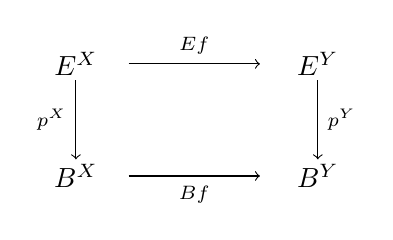
\begin{tikzpicture}[x=1.9em,y=1.5em]
  \node (EX) at (0,1.3)  {$E^{X}$};
  \node (EY) at (4.6,1.3){$E^{Y}$};
  \node (BX) at (0,-1.4) {$B^{X}$};
  \node (BY) at (4.6,-1.4){$B^{Y}$};
  \draw[->] (1.0,1.3) -- node[above]{$\scriptstyle Ef$} (3.5,1.3);
  \draw[->] (0,0.9) -- node[left]{$\scriptstyle p^{X}$} (0,-1.0);
  \draw[->] (4.6,0.9) -- node[right]{$\scriptstyle p^{Y}$} (4.6,-1.0);
  \draw[->] (1.0,-1.4) -- node[below]{$\scriptstyle Bf$} (3.5,-1.4);
\end{tikzpicture}
\end{center}
特别地，$p^{X}$-\trCartesianArrow{}都是逐点 $p$-笛卡尔的。反之，任何逐点 $p$-笛卡尔
柱面都经由一个逐点同构穿过一支 $p^{X}$-\trCartesianArrow{}而分解。由
\cref{cor:exponential-ideal}，逐点同构实际上就是同构，故由 $p^{X}$-\trCartesianArrow{}%
的同构稳定性，任何逐点 $p$-笛卡尔柱面都是一支 $p^{X}$-\trCartesianArrow。
\end{proof}

下述\trLifting{}性质将用于证明\cref{prop:cocartesian-rari-terminal-elements}。

\begin{lemma}\label{lem:cylinder-lifting-property}
设 $X\hookrightarrow Y$ 是单纯集 $Y$ 的一个单纯子集。
\begin{enumerate}[label=(\roman*)]
\item 任何 $n\ge 0$ 的\trLifting{}问题
\begin{center}
\begin{tikzpicture}[x=1.9em,y=1.4em]
  \node (u) at (0,1.3)    {$X\times\Delta[1]\cup Y\times\{1\}$};
  \node (E) at (7.0,1.3)  {$E$};
  \node (l) at (0,-1.4)   {$Y\times\Delta[1]$};
  \node (B) at (7.0,-1.4) {$B$};
  \draw[->] (3.6,1.3) -- node[above]{$\scriptstyle e$} (6.2,1.3);
  \draw[right hook->] (0,0.9) -- (0,-1.0);
  \draw[->,dashed] (0.8,-1.2) -- (6.2,1.05);
  \node at (3.4,-0.4) {$\scriptstyle\bar{e}$};
  \draw[->] (7.0,0.95) -- node[right]{$\scriptstyle p$} (7.0,-1.0);
  \draw[->] (2.6,-1.4) -- node[below]{$\scriptstyle b$} (5.6,-1.4);
\end{tikzpicture}
\end{center}
其中柱面
$X\times\Delta[1]\subseteq X\times\Delta[1]\cup Y\times\{1\}\xrightarrow{\ e\ }E$
是逐点 $p$-笛卡尔的，都容有一个解 $\bar{e}$，且该解同样是逐点 $p$-笛卡尔的。
\item 任何 $n\ge 1$ 的\trLifting{}问题
\begin{center}
\begin{tikzpicture}[x=1.9em,y=1.4em]
  \node (u) at (0,1.3)    {$X\times\Delta[n]\cup Y\times\Lambda^{n}[n]$};
  \node (E) at (7.0,1.3)  {$E$};
  \node (l) at (0,-1.4)   {$Y\times\Delta[n]$};
  \node (B) at (7.0,-1.4) {$B$};
  \draw[->] (4.3,1.3) -- node[above]{$\scriptstyle e$} (6.2,1.3);
  \draw[right hook->] (0,0.9) -- (0,-1.0);
  \draw[->,dashed] (0.8,-1.2) -- (6.2,1.05);
  \node at (3.4,-0.4) {$\scriptstyle\bar{e}$};
  \draw[->] (7.0,0.95) -- node[right]{$\scriptstyle p$} (7.0,-1.0);
  \draw[->] (2.4,-1.4) -- node[below]{$\scriptstyle b$} (5.6,-1.4);
\end{tikzpicture}
\end{center}
其中柱面
$Y\times\Delta^{\{n-1,n\}}\subseteq X\times\Delta[n]\cup Y\times\Lambda^{n}[n]\xrightarrow{\ e\ }E$
是逐点 $p$-笛卡尔的，都容有一个解 $\bar{e}$。
\end{enumerate}
\end{lemma}

\begin{proof}
带 $X\hookrightarrow Y$ 的\trLeibnizTensor{}定义了一个函子
$\sSet^{2}\to\sSet^{2}$，它保持收缩图 \eqref{eq:horn-inclusion-retract}，故
(ii) 的\trLifting{}性质由 (i) 得出。而 (i) 的\trLifting{}性质则归纳地由
\cref{prop:cartesian-arrow-analytic}(vi) 结合「任何单态射 $X\hookrightarrow Y$
都可以分解为诸包含 $i_{n}\colon\partial\Delta[n]\hookrightarrow\Delta[n]$ 之
余积的推出的一个序列复合」这一事实得出；并且由
\cref{prop:leibniz-construction-preserves}(vii)，再与
$\{1\}\hookrightarrow\Delta[1]$ 作推出积，便同样给出诸推出积
$\partial\Delta[n]\times\Delta[1]\cup\Delta[n]\times\{1\}\hookrightarrow\Delta[n]\times\Delta[1]$
之余积的推出的一个序列复合。
\end{proof}

最后一个结果表明，拟范畴之间的\trDiscreteCocartesianFibration{}与\trDiscreteCartesianFibration，分别与
Joyal \cite{bib61} 所引入的\trLeftFibration{}类与\trRightFibration{}类相重合。

\begin{proposition}\label{prop:discrete-cartesian-analytic}
对拟范畴之间的一条\trIsofibration{} $p\colon E\twoheadrightarrow B$，以下诸
条件等价，并且定义了 $p$ 成为一条\textbf{\trDiscreteCartesianFibration}的含义：
\begin{enumerate}[label=(\roman*)]
\item 映射 $p\colon E\twoheadrightarrow B$ 是一条\trCartesianFibration，其诸%
\trFiber{}皆为\trKanComplex。
\item \trQuasiCategory{}的\trHomotopyTwoCategory{}中的每个 2-\trCell{}
$\beta\colon b\Rightarrow pe$ 都容有一个本质唯一的提升：给定
$\chi\colon e'\Rightarrow e$ 与 $\psi\colon e''\Rightarrow e$ 使得
$p\chi=p\psi=\beta$，则存在一个\trIsomorphism{} $\gamma\colon e''\Rightarrow e'$，
使得 $\chi\cdot\gamma=\psi$ 且 $p\gamma=\mathrm{id}$。
\item 诱导函子 $i_{1}\hat{p}\colon E^{2}\twoheadrightarrow\mathrm{Hom}_{B}(B,p)$
是一条\trTrivialFibration。
\item 函子 $p\colon E\to B$ 是一个\trRightFibration，即带有如下\trLifting{}性质：
\begin{center}
\begin{tikzpicture}[x=1.9em,y=1.4em]
  \node (ho) at (0,1.3)   {$\Lambda^{k}[n]$};
  \node (E)  at (3.6,1.3) {$E$};
  \node (dn) at (0,-1.4)  {$\Delta[n]$};
  \node (B)  at (3.6,-1.4){$B$};
  \draw[->] (1.0,1.3) -- (2.8,1.3);
  \draw[right hook->] (0,0.95) -- (0,-0.9);
  \draw[->,dashed] (0.45,-1.2) -- (3.1,1.05);
  \draw[->] (3.6,0.95) -- node[right]{$\scriptstyle p$} (3.6,-1.0);
  \draw[->] (1.0,-1.4) -- (2.8,-1.4);
  \node at (6.1,0) {对 $n\ge 0$ 与 $0<k\le n$。};
\end{tikzpicture}
\end{center}
\end{enumerate}
\end{proposition}

\begin{proof}
第一个刻画 (i) 是把原来的\cref{def:discrete-co-cartesian-fibration}借
\cref{prop:discrete-fibers-isofibration}重新解读——后者说：一条\trIsofibration{}
$p\colon E\twoheadrightarrow B$ 在 $\QCat_{/B}$ 中定义一个\trDiscrete{}对象，
当且仅当其诸\trFiber{}是\trKanComplex。(i) 与 (ii) 的等价性证明于
\cref{prop:discrete-cartesian-characterization}，而 (i) 与 (iii) 的等价性则
证明于\cref{prop:internal-characterization-discrete}。

我们最后证明 (iii) 与 (iv) 的等价性。经伴随，$i_{1}\hat{p}$ 是一条%
\trTrivialFibration，当且仅当如下右方的\trLifting{}问题有解
\begin{center}
\begin{tikzpicture}[x=1.9em,y=1.4em]
  \node (pd) at (0,1.3)    {$\partial\Delta[n]$};
  \node (E2) at (3.4,1.3)  {$E^{2}$};
  \node (dn) at (0,-1.4)   {$\Delta[n]$};
  \node (H)  at (3.4,-1.4) {$\mathrm{Hom}_{B}(B,p)$};
  \draw[->] (1.0,1.3) -- (2.3,1.3);
  \draw[right hook->] (0,0.95) -- (0,-0.9);
  \draw[->,dashed] (0.5,-1.2) -- (2.9,1.05);
  \draw[->] (3.4,0.95) -- node[right]{$\scriptstyle i_{1}\hat{p}$} (3.4,-1.0);
  \draw[->] (1.0,-1.4) -- (2.1,-1.4);
  \node at (5.2,0) {$\;\leftrightsquigarrow\;$};
  \begin{scope}[shift={(7.8,0)}]
    \node (u) at (0,1.3)    {$\partial\Delta[n]\times\Delta[1]\cup\Delta[n]\times\{1\}$};
    \node (E) at (6.6,1.3)  {$E$};
    \node (l) at (0,-1.4)   {$\Delta[n]\times\Delta[1]$};
    \node (B) at (6.6,-1.4) {$B$};
    \draw[->] (4.6,1.3) -- (5.8,1.3);
    \draw[right hook->] (0,0.9) -- (0,-1.0);
    \draw[->,dashed] (0.8,-1.2) -- (5.9,1.05);
    \draw[->] (6.6,0.95) -- node[right]{$\scriptstyle p$} (6.6,-1.0);
    \draw[->] (3.0,-1.4) -- (5.4,-1.4);
  \end{scope}
\end{tikzpicture}
\end{center}
由\cref{prop:leibniz-marked-anodyne}，若 $p\colon E\to B$ 是一个满足条件 (iv)
的\trRightFibration，则如上右方的\trLifting{}问题容有一个解，从而
$i_{1}\hat{p}\colon E^{2}\twoheadrightarrow\mathrm{Hom}_{B}(B,p)$ 是一条%
\trTrivialFibration，即证得 (iii)。反之，对 $0<k\le n$，号角包含
$\Lambda^{k}[n]\hookrightarrow\Delta[n]$ 是一个收缩
\begin{center}
\begin{tikzpicture}[x=1.9em,y=1.5em]
  \node (a) at (0,1.3)    {$\Lambda^{k}[n]$};
  \node (b) at (5.0,1.3)  {$\Lambda^{k}[n]\times\Delta[1]\cup\Delta[n]\times\{1\}$};
  \node (c) at (11.4,1.3) {$\Lambda^{k}[n]$};
  \node (d) at (0,-1.6)   {$\Delta[n]$};
  \node (e) at (5.0,-1.6) {$\Delta[n]\times\Delta[1]$};
  \node (f) at (11.4,-1.6){$\Delta[n]$};
  \draw[right hook->] (1.0,1.3) -- node[above]{$\scriptstyle\Lambda^{k}[n]\times\{0\}$} (2.4,1.3);
  \draw[->] (8.4,1.3) -- node[above]{$\scriptstyle r$} (10.3,1.3);
  \draw[right hook->] (1.0,-1.6) -- node[above]{$\scriptstyle\Delta[n]\times\{0\}$} (2.9,-1.6);
  \draw[->] (7.6,-1.6) -- node[above]{$\scriptstyle r$} (10.3,-1.6);
  \draw[right hook->] (0,0.9) -- (0,-1.1);
  \draw[right hook->] (5.0,0.8) -- (5.0,-1.1);
  \draw[right hook->] (11.4,0.9) -- (11.4,-1.1);
\end{tikzpicture}
\end{center}
其中 $r(i,0)=i$，而
$r(i,1)=\begin{cases}i & i\ne k-1\\ k & i=k-1\end{cases}$。于是，要求解 (iv)
所假定的那一\trLifting{}问题，只需证明 $p$ 对推出积
$(\Lambda^{k}[n]\hookrightarrow\Delta[n])\mathbin{\widehat{\times}}(\{1\}\hookrightarrow\Delta[1])$
容有提升；而后者经转置便成为单态射
$\Lambda^{k}[n]\hookrightarrow\Delta[n]$ 与
$i_{1}\hat{p}\colon E^{2}\twoheadrightarrow\mathrm{Hom}_{B}(B,p)$ 之间的一个%
\trLifting{}问题。若 (iii) 成立且 $i_{1}\hat{p}$ 是一条\trTrivialFibration，
那么这就构造出所求的提升。
\end{proof}

\subsection*{练习}

\begin{exercise}\label{ex:inner-fibration-isofibration}
设 $p\colon E\to B$ 是拟范畴之间的一个\trInnerFibration，使得 $B$ 中任何 1-\trSimplex{}
$\beta\colon b\to pe$ 都容有 $E$ 中的一个提升 $\chi\colon e'\to e$，使得任何
$n\ge 2$ 的\trLifting{}问题
\begin{center}
\begin{tikzpicture}[x=1.9em,y=1.4em]
  \node (d1) at (0,1.3)    {$\Delta[1]$};
  \node (ho) at (3.6,1.3)  {$\Lambda^{n}[n]$};
  \node (E)  at (7.4,1.3)  {$E$};
  \node (dn) at (3.6,-1.4) {$\Delta[n]$};
  \node (B)  at (7.4,-1.4) {$B$};
  \draw[->] (1.0,1.3) -- node[below]{$\scriptstyle\{n-1,n\}$} (2.6,1.3);
  \draw[->] (4.6,1.3) -- (6.4,1.3);
  \draw[->] (0.6,1.8) to[bend left=20] node[above,pos=0.5]{$\scriptstyle\chi$} (6.8,1.8);
  \draw[right hook->] (3.6,0.95) -- (3.6,-0.9);
  \draw[->,dashed] (4.0,-1.2) -- (6.9,1.0);
  \draw[->] (7.4,0.95) -- node[right]{$\scriptstyle p$} (7.4,-0.9);
  \draw[->] (4.6,-1.4) -- (6.4,-1.4);
\end{tikzpicture}
\end{center}
都有解。证明 $p$ 是一个\trIsofibration。
\end{exercise}

\begin{exercise}\label{ex:cocartesian-equivalences}
陈述并证明下述诸对象的多种综合定义与解析定义之间的等价：
\begin{enumerate}[label=(\roman*)]
\item 拟范畴之间的一条余笛卡尔纤维化；
\item 拟范畴中的一支\trCocartesianArrow（cocartesian arrow）；
\item 拟范畴之间的一条\trDiscreteCocartesianFibration。
\end{enumerate}
\end{exercise}

   %

\providecommand{\QCat}{\mathcal{Q}\mathit{Cat}}%
\providecommand{\hQCat}{\mathfrak{h}\QCat}%
\providecommand{\Hom}{\operatorname{Hom}}%

\section{伴随}\label{sec:f-adjunctions}

拟范畴间伴随的解析定义与综合定义之间的比较，比本附录中所考察的其他范畴论
概念要微妙一些，因为这两者通常是以不同的数据来陈述的。伴随的综合定义原本
归于 Joyal \cite{bib63}，它涉及两个指定的函子 $f\colon B\to A$ 与
$u\colon A\to B$，连同指定的映射 $\eta\colon B\times\Delta[1]\to B$ 与
$\epsilon\colon A\times\Delta[1]\to A$\footnote{原书两处均印作「$\eta$」；
按\cref{prop:synthetic-analytic-adjunction}(i) 中 $\eta\colon\mathrm{id}_{B}\Rightarrow uf$
与 $\epsilon\colon fu\Rightarrow\mathrm{id}_{A}$ 之记号分工，第二处疑为
$\epsilon$ 之误，此处径改。——译者注}——在 $B^{B}$ 或 $A^{A}$ 中至差一个
同伦——再连同拟范畴 $B^{A}$ 与 $A^{B}$ 中见证\trTriangleEqualities{}的
2-\trSimplex{}。与此相对，$A$ 与 $B$ 之间伴随的解析概念归于 Lurie
\cite[5.2.2.1]{bib78}，它被定义为一条等价纤维化\footnote{爱挑剔的读者或许
会注意到，Lurie 只要求一个\trInnerFibration，但 $\Delta[1]$ 之上的任何\trInnerFibration{}都
自动是等价纤维化。事实上，只要 $M$ 是一个拟范畴，任何单纯映射
$M\to\Delta[1]$ 都自动是等价纤维化。} $M\twoheadrightarrow\Delta[1]$，它
同时是一条\trCartesianFibration{}与一条\trCocartesianFibration，称为一个
\textbf{\trCorrespondence}（correspondence），并配有等价 $M_{1}\simeq A$ 与
$M_{0}\simeq B$，把拟范畴 $A$ 与 $B$ 等同于该 1-\trSimplex{}两端点之上的
诸\trFiber。

由于\cref{prop:adjunction-equivalence-invariant}证明了伴随的综合概念是等价
不变的，我们稍微简化一下记号，令 $B$ 与 $A$ 表示等价纤维化
$M\twoheadrightarrow\Delta[1]$ 在 0 与 1 之上的诸\trFiber。本节的目标是
证明：从一条余笛卡尔与笛卡尔纤维化 $M\twoheadrightarrow\Delta[1]$ 出发，
可以提取出一个 $B$ 与 $A$ 之间的\trAdjunction，其伴随函子在\trIsomorphism{}%
的意义下被唯一确定；反之，从一个 2-范畴式的\trAdjunction{}出发，可以构造出
一个相应的\trCorrespondence{} $M\twoheadrightarrow\Delta[1]$，其在\trFiberedEquivalence{}%
的意义下唯一。由于证明更为繁难，我们把论证拆成若干个中间步骤。

\begin{proposition}\label{prop:correspondence-adjunction}
设 $M$ 是一个配有映射 $M\twoheadrightarrow\Delta[1]$ 的\trQuasiCategory，
该映射同时是一条\trCocartesianFibration{}与\trCartesianFibration。那么
\begin{itemize}
\item 诸\trFiber{} $B\coloneqq M_{0}$ 与 $A\coloneqq M_{1}$，以及
\item 由 $\Delta[1]$ 中泛箭头的余笛卡尔\trLifting{}与笛卡尔\trLifting{}%
分别定义的诸\trFunctor{} $f\colon B\to A$ 与 $u\colon A\to B$
\end{itemize}
定义一个\trAdjunction
\begin{center}
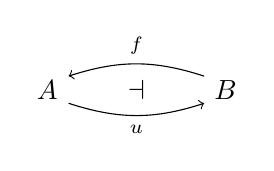
\begin{tikzpicture}[x=1.4em,y=1.4em]
  \node (A) at (0,0)   {$A$};
  \node (B) at (4.6,0) {$B$};
  \draw[->] (4.05,0.35) to[bend right=18] node[above]{$\scriptstyle f$} (0.55,0.35);
  \node at (2.3,0) {$\dashv$};
  \draw[->] (0.55,-0.35) to[bend right=18] node[below]{$\scriptstyle u$} (4.05,-0.35);
\end{tikzpicture}
\end{center}
\end{proposition}

\begin{proof}
这是\cref{prop:bifibration-fibered-adjunction}的一个特例。我们回顾 $f$ 与
$u$ 的构造，而把其余细节留给该结果与\cref{rem:fiber-action}。设 $\chi$
表示 $\Delta[1]$ 中泛箭头的一支余笛卡尔\trLifting，其定义域是 0 之上的%
\trFiber{}之包含 $B\hookrightarrow M$。这条被提升箭头的陪域落入 1 之上
的\trFiber{}之中，从而经该\trFiber{}的包含 $A\hookrightarrow M$ 唯一地分解：
\begin{center}
\begin{tikzpicture}[x=1.9em,y=1.5em]
  \node (B)  at (0,1.4)    {$B$};
  \node (M)  at (3.2,1.4)  {$M$};
  \node (One) at (0,-1.4)  {$1$};
  \node (D1) at (3.2,-1.4) {$\Delta[1]$};
  \draw[->] (0.45,1.85) to[bend left=20] (2.75,1.85);
  \node at (0.55,0.8) {$\scriptstyle\llcorner$};
  \draw[->] (0,1.0) -- (0,-1.0);
  \draw[->] (3.2,1.0) -- (3.2,-1.0);
  \draw[->] (0.6,-1.05) to[bend left=22] node[above]{$\scriptstyle 0$} (2.6,-1.05);
  \node at (1.6,-1.5) {$\scriptstyle\Downarrow\psi$};
  \draw[->] (0.6,-1.8) -- node[below]{$\scriptstyle 1$} (2.6,-1.8);
  \node at (5.1,0) {$=$};
  \begin{scope}[shift={(7.0,0)}]
  \node (B2) at (0,1.4)    {$B$};
  \node (M2) at (3.2,1.4)  {$M$};
  \node (Ax) at (1.6,0.1)  {$A$};
  \node (O2) at (0,-1.4)   {$1$};
  \node (D2) at (3.2,-1.4) {$\Delta[1]$};
  \draw[->,dashed] (0.45,1.85) to[bend left=20] node[above]{$\scriptstyle\psi\chi$} (2.75,1.85);
  \draw[->] (0.35,0.95) -- node[left,pos=0.55]{$\scriptstyle f$} (1.25,0.42);
  \draw[right hook->] (1.95,0.42) -- (2.9,1.0);
  \node at (2.5,0.55) {$\scriptstyle\llcorner$};
  \draw[->] (0,1.0) -- (0,-1.0);
  \draw[->] (3.2,1.0) -- (3.2,-1.0);
  \draw[->] (0.6,-1.05) to[bend left=22] node[below]{$\scriptstyle 1$} (2.6,-1.05);
  \end{scope}
\end{tikzpicture}
\end{center}
这一分解定义了\trFunctor{} $f\colon B\to A$。由于一支固定箭头的诸余笛卡尔%
\trLifting{}与一个固定\trFunctor{}的诸\trAdjunction{}各自都在%
\trIsomorphism{}的意义下唯一，这一构造是适当良定义的。\trRightAdjoint{}
$u\colon A\to B$ 的构造是对偶的，涉及 $\Delta[1]$ 中泛箭头的一支笛卡尔%
\trLifting。
\end{proof}

逆命题用到了我们称为\textbf{拟范畴\trCollage{}构造}（quasi-categorical collage
construction）的东西。

\begin{definition}[拟范畴\trCollage{}构造]\label{def:quasicategorical-collage}
对拟范畴之间的任意余跨度 $B\xrightarrow{g}C\xleftarrow{f}A$\footnote{原书两杆
均印作指向左，与定义条件及 p.728 证明之 $g\colon B\to C$ 不合，此处径改。
——译者注}，定义一个单纯集
$\mathrm{col}(f,g)$ 如下：
\[
\mathrm{col}(f,g)_{n}=\Bigl\{(a\in A_{i},\,b\in B_{j},\,c\in C_{n})\;\Bigm|\;
\begin{array}{l}
c_{[0,\dotsc,i]}=f(a),\ i,j\ge -1,\\
c_{[n-j,\dotsc,n]}=g(b),\ i+j=n-1
\end{array}\Bigr\}
\]
其中约定由 $\Delta[-1]$ 编号的条件为空（或者说每个单纯集都是末端增广的）。
有显然的包含纳入如下交换图：
\begin{center}
\begin{tikzpicture}[x=1.9em,y=1.5em]
  \node (B)  at (0,1.4)    {$B$};
  \node (C)  at (3.4,1.4)  {$\mathrm{col}(f,g)$};
  \node (A)  at (6.8,1.4)  {$A$};
  \node (B1) at (0,-1.4)   {$\{1\}$};
  \node (D)  at (3.4,-1.4) {$\Delta[1]$};
  \node (Z)  at (6.8,-1.4) {$\{0\}$};
  \draw[right hook->] (0.5,1.4) -- (2.2,1.4);
  \draw[right hook->] (6.3,1.4) -- (4.6,1.4);
  \node at (0.65,0.75) {$\scriptstyle\llcorner$};
  \node at (6.15,0.75) {$\scriptstyle\llcorner$};
  \draw[->] (0,1.0) -- (0,-1.0);
  \draw[->] (3.4,1.0) -- (3.4,-1.0);
  \node at (3.85,0) {$\scriptstyle\rho$};
  \draw[->] (6.8,1.0) -- (6.8,-1.0);
  \draw[right hook->] (0.5,-1.4) -- (2.2,-1.4);
  \draw[right hook->] (6.3,-1.4) -- (4.6,-1.4);
\end{tikzpicture}
\end{center}
映射 $\rho$ 把 $n$ 单形 $(a\colon\Delta[i]\to A,\ b\colon\Delta[j]\to B,\ c\colon\Delta[n]\to C)$
送到把 $0,\dotsc,i$ 送到 0 而把 $i+1,\dotsc,n$ 送到 1 的那个 $n$ 单形
$[n]\to[1]$。注意，$\rho$ 在 0 之上的\trFiber{}\trIsomorphism{}于 $A$，而
$\rho$ 在 1 之上的\trFiber{}\trIsomorphism{}于 $B$。
\end{definition}

按照我们对\trTwoSidedFibration{}与\trModule{}的惯例，我们记 $B+A\hookrightarrow\mathrm{col}(f,g)$
为 1 与 0 之上的诸\trFiber{}之包含——1 之上的\trFiber{}在左，0 之上的%
\trFiber{}在右。这就把协变地作用的拟范畴置于「左」，而把反变地作用的拟范畴
置于「右」。

\begin{lemma}\label{lem:collage-inner-fibration}
映射 $\rho\colon\mathrm{col}(f,g)\to\Delta[1]$ 是一个\trInnerFibration。特别地，单纯集
$\mathrm{col}(f,g)$ 是一个\trQuasiCategory。
\end{lemma}

\begin{proof}
由于 $\rho$ 在 0 与 1 之上的诸\trFiber{}是拟范畴 $A$ 与 $B$，只需考虑内号角
\begin{center}
\begin{tikzpicture}[x=1.9em,y=1.5em]
  \node (L)  at (0,1.3)    {$\Lambda^{k}[n]$};
  \node (Cl) at (4.4,1.3)  {$\mathrm{col}(f,g)$};
  \node (Dn) at (0,-1.4)   {$\Delta[n]$};
  \node (D1) at (4.4,-1.4) {$\Delta[1]$};
  \draw[->] (1.2,1.3) -- (3.0,1.3);
  \draw[right hook->] (0,0.95) -- (0,-1.0);
  \draw[->] (1.2,-1.4) -- node[below]{$\scriptstyle\alpha$} (3.3,-1.4);
  \draw[->] (4.4,0.95) -- (4.4,-1.0);
  \node at (4.85,0) {$\scriptstyle\rho$};
  \draw[->,dashed] (0.5,-1.15) -- (3.9,1.05);
\end{tikzpicture}
\end{center}
其中 $\alpha\colon[n]\to[1]$ 是满射。设 $\alpha$ 把 $0,\dotsc,i$ 送到 0，把
$i+1,\dotsc,n$ 送到 1。注意，对任何 $0<k<n$，$\Delta[n]$ 的诸面
$\{0,\dotsc,i\}$ 与 $\{i+1,\dotsc,n\}$ 都属于号角 $\Lambda^{k}[n]$。特别地，
映射 $\Lambda^{k}[n]\to\mathrm{col}(f,g)$ 把单纯形 $a\colon\Delta[i]\to A$
与 $b\colon\Delta[n-i-1]\to B$ 连同一个号角 $\Lambda^{k}[n]\to C$ 一道等同
起来，该号角的初始面与最终面是这些单纯形在 $f\colon A\to C$ 与
$g\colon B\to C$ 之下的像。由于 $C$ 是拟范畴，这个号角容有一个填充体
$c\colon\Delta[n]\to C$，而三元组 $(a,b,c)$ 定义出 $\mathrm{col}(f,g)$ 中
解决该\trLifting{}问题的一个 $n$ 单形。
\end{proof}

我们记 $\mathrm{col}(f,B)$ 为 $f\colon A\to B$ 与 $B$ 上的恒同所成的\trCollage。

\begin{lemma}\label{lem:collage-cocartesian-fibration}
对任何 $f\colon A\to B$，映射 $\rho\colon\mathrm{col}(f,B)\to\Delta[1]$ 是
一条\trCocartesianFibration。
\end{lemma}

\begin{proof}
由\cref{prop:cartesian-fibration-analytic}(vi)，为证明本断言，我们只需指定
$\Delta[1]$ 的非退化 1-\trSimplex{}的诸余笛卡尔\trLifting，并证明这些边具有
相应的\trUniversalProperty。为此，对任何顶点 $a\in A_{0}$，设
$\chi_{a}\colon\Delta[1]\to\mathrm{col}(f,B)$ 是 1-\trSimplex
\[
\chi_{a}\coloneqq(a\colon\Delta[0]\to A,\ fa\colon\Delta[0]\to B,\ fa\sigma^{0}\colon\Delta[1]\to B),
\]
它由位于 $\Delta[1]$ 中该 1-\trSimplex{}之上的、$fa\in B_{0}$ 处的退化边
给出。为证 $\chi_{a}$ 是 $\rho$-\trCocartesian，我们必须为任何以 $\chi_{a}$
为初始边的左号角构造填充体
\begin{center}
\begin{tikzpicture}[x=1.9em,y=1.5em]
  \node (D1) at (0,1.3)    {$\Delta[1]$};
  \node (L)  at (3.6,1.3)  {$\Lambda^{0}[n]$};
  \node (Cl) at (7.6,1.3)  {$\mathrm{col}(f,B)$};
  \node (Dn) at (3.6,-1.4) {$\Delta[n]$};
  \node (D2) at (7.6,-1.4) {$\Delta[1]$};
  \draw[->] (1.1,1.3) -- node[below]{$\scriptstyle\{0,1\}$} (2.5,1.3);
  \draw[->] (4.7,1.3) -- (6.5,1.3);
  \draw[->] (0.5,1.8) to[bend left=18] node[above,pos=0.5]{$\scriptstyle\chi_{a}$} (7.1,1.8);
  \draw[right hook->] (3.6,0.95) -- (3.6,-1.0);
  \draw[->] (4.7,-1.4) -- node[below]{$\scriptstyle\beta$} (6.5,-1.4);
  \draw[->] (7.6,0.95) -- (7.6,-1.0);
  \node at (8.05,0) {$\scriptstyle\rho$};
  \draw[->,dashed] (4.0,-1.15) -- (7.1,1.05);
\end{tikzpicture}
\end{center}
注意，这一条件蕴含底映射 $\beta\colon[n]\to[1]$ 把 0 送到 0，而把其余顶点
送到 1。映射 $\Lambda^{0}[n]\to\mathrm{col}(f,B)$ 在拟范畴 $B$ 中定义了一个
号角 $\Lambda^{0}[n]\to B$，其首条边是退化的。由
\cref{prop:special-outer-horn-filling}，这个「特殊外号角」容有一个填充体
$b\colon\Delta[n]\to B$，而三元组
\[
(a\colon\Delta[0]\to A,\ b\sigma^{0}\colon\Delta[n-1]\to B,\ b\colon\Delta[n]\to B)
\]
定义出解决该\trLifting{}问题的 $\mathrm{col}(f,B)$ 中的一个 $n$ 单形。
\end{proof}

\begin{proposition}\label{prop:collage-oplax-colimit}
对拟范畴之间的任何 $f\colon A\to B$，\trCollage{} $\mathrm{col}(f,B)$ 定义 $f$ 在
$\QCat$ 中的\textbf{\trOplaxColimit}（oplax colimit）。也就是说，
$\mathrm{col}(f,B)$ 在如下推出图之下定义一个锥\footnote{图中虚线杆之标目
原书印作 $i_{1}\hat{p}$，与本页正文「诱导映射 $k$」不合（本节并无 F.4 节之
$E^{2}\twoheadrightarrow\mathrm{Hom}_{B}(B,p)$ 语境），疑为 F.4 节同名记号
之排印残留，此处照录原书面貌。——译者注}
\begin{center}
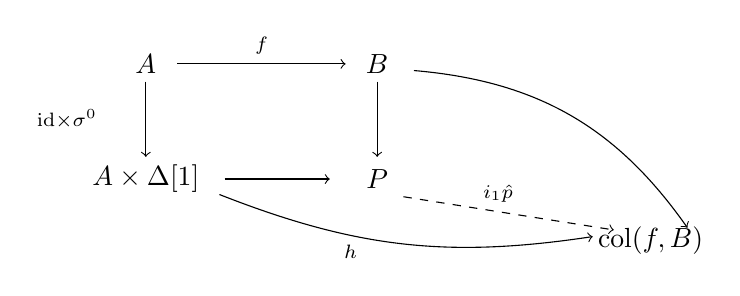
\begin{tikzpicture}[x=1.9em,y=1.6em]
  \node (A)  at (0,1.4)    {$A$};
  \node (B)  at (4.4,1.4)  {$B$};
  \node (AD) at (0,-1.2)   {$A\times\Delta[1]$};
  \node (P)  at (4.4,-1.2) {$P$};
  \node (Cl) at (9.6,-2.6) {$\mathrm{col}(f,B)$};
  \draw[->] (0.6,1.4) -- node[above]{$\scriptstyle f$} (3.8,1.4);
  \draw[->] (0,1.0) -- (0,-0.7);
  \node at (-1.5,0.15) {$\scriptstyle\mathrm{id}\times\sigma^{0}$};
  \draw[->] (4.4,1.0) -- (4.4,-0.7);
  \node at (2.9,0.35) {$\scriptstyle\llcorner$};
  \draw[->] (1.5,-1.2) -- (3.5,-1.2);
  \draw[->] (1.4,-1.55) to[bend right=15] node[below,pos=0.35]{$\scriptstyle h$} (8.5,-2.5);
  \draw[->] (5.1,1.25) to[bend left=25] (10.3,-2.3);
  \draw[->,dashed] (4.9,-1.6) -- node[above,pos=0.45]{$\scriptstyle i_{1}\hat{p}$} (8.9,-2.35);
\end{tikzpicture}
\end{center}
使得诱导映射 $k$ 是\trInnerAnodyne{}的，从而特别是在 Joyal \trModelStructure{}中
的一个\trWeakEquivalence。
\end{proposition}

\begin{proof}
映射 $k$ 是映射 $h$ 的一个商，后者有如下显式描述。对每个 $n$ 单形
$(a,\alpha)\colon\Delta[n]\to A\times\Delta[1]$，定义
$i\coloneqq\lvert\alpha^{-1}(0)\rvert-1$，从而 $-1\le i\le n$。那么 $h$ 把
$(a,\alpha)$ 送到 $\mathrm{col}(f,B)$ 的由如下三元组所对应的 $n$ 单形
\[
(a|_{[0,\dotsc,i]}\colon\Delta[i]\to A,\ fa|_{[i+1,\dotsc,n]}\colon\Delta[n-i-1]\to B,\ fa\colon\Delta[n]\to B).
\]
注意，复合 $\rho h\colon A\times\Delta[1]\to\Delta[1]$ 是投影。

剩下要做的是把 $k$ 呈现为内号角包含之余积的推出的一个序列复合。为此，首先
注意
\[
\mathrm{col}(f,B)_{n}=A_{n}\sqcup A_{n-1}\times_{B_{n-1}}B_{n}\sqcup\dotsb\sqcup A_{0}\times_{B_{0}}B_{n}\sqcup B_{n}
\]
其中每个映射 $B_{n}\to B_{i}$ 是对应于 $\{0,\dotsc,i\}\hookrightarrow\Delta[i]$
的初始面映射。在这一分解的视角下，$P_{n}$ 是这样一个子集：它含有诸集合
$A_{n}$ 与 $B_{n}$，以及 $A_{i}\times_{B_{i}}B_{n}$ 中其在 $B_{n}$ 中的分量
落在 $f$ 的像内的那个子集。$\mathrm{col}(f,B)$ 中尚待贴附的诸 $n$ 单形对应
于 $A_{i}\times_{B_{i}}B_{n}$（$0\le i<n$）中不属于刚才所论意义上的 $f$ 之
像的那些元素。特别值得注意的是，顶点上的映射
$k\colon P_{0}\hookrightarrow\mathrm{col}(f,B)_{0}$ 是一个\trIsomorphism，
而对一切 $n\ge 1$，$k\colon P_{n}\hookrightarrow\mathrm{col}(f,B)_{n}$ 是
一个单射。

为枚举我们的贴附映射，我们从 $\mathrm{col}(f,B)$ 中非退化的诸 $n$ 单形
（$n\ge 1$）不在 $f$ 的像内者的集合出发，并再剔除 $A_{i}\times_{B_{i}}B_{n}$
中其分量 $b\in B_{n}$ 落在退化映射 $\sigma_{i}\colon B_{n-1}\to B_{n}$ 的像
内的那些元素。将这一单纯形集合先按 $n$ 递增的顺序、继而按标号 $i$ 递增的
顺序偏序化；也就是说，我们对二元组 $(n,i)$（$n\ge 1$，$0\le i<n$）之集合
按字典序排序。

我们把包含 $P\hookrightarrow\mathrm{col}(f,B)$ 滤过为
\[
\begin{gathered}
P\hookrightarrow P_{(1,0)}\hookrightarrow P_{(2,0)}\hookrightarrow P_{(2,1)}\hookrightarrow P_{(3,0)}\hookrightarrow\dotsb\\
\dotsb\hookrightarrow P_{(n,i)}\hookrightarrow\dotsb\hookrightarrow\mathrm{colim}\simeq\mathrm{col}(f,B)
\end{gathered}
\]
其中单纯集 $P_{(n,i)}$ 由前一个经一个推出构造而得，该推出所用的内号角之
余积以 $b$ 不在 $f$ 或 $\sigma_{i}$ 的像内的诸 $n$ 单形
$(a,b)\in A_{i}\times_{B_{i}}B_{n}$ 之集合为指标。以 $(a,b)$ 为标目的号角之
填充体将把这个 $n$ 单形作为号角的缺失面贴附到 $B_{n}$ 上，并且同时贴附
$n+1$ 单形 $(a,b\sigma^{i})\in A_{i}\times_{B_{i}}B_{n+1}$。

考虑一个 $b$ 不在 $f$ 或 $\sigma_{i}$ 的像内的单纯形
$(a,b)\in A_{i}\times_{B_{i}}B_{n}$。定义一个号角
\begin{center}
\begin{tikzpicture}[x=1.9em,y=1.5em]
  \node (L)  at (0,1.3)    {$\Lambda^{i+1}[n+1]$};
  \node (P)  at (5.8,1.3)  {$P_{(n,i)}$};
  \node (D)  at (0,-1.5)   {$\Delta[n+1]$};
  \node (Cl) at (5.8,-1.5) {$\mathrm{col}(f,B)$};
  \draw[->] (2.6,1.3) -- (4.4,1.3);
  \draw[right hook->] (0,0.95) -- (0,-1.1);
  \draw[right hook->] (5.8,0.95) -- (5.8,-1.1);
  \draw[->] (1.7,-1.5) -- node[below]{$\scriptstyle(a,b\sigma^{i})$} (4.4,-1.5);
\end{tikzpicture}
\end{center}
对每个 $0\le j<i+1$，$n+1$ 单形 $(a,b\sigma^{i})$ 的 $\delta^{j}$ 面是
$n$ 单形 $(a\delta^{j},\,b\sigma^{i}\delta^{j})$，它落于 $P_{(n,i-1)}$ 之中，
或在 $i=0$ 的情形落于 $B\hookrightarrow P$ 之中。对每个 $i+1<j\le n+1$，
$n+1$ 单形 $(a,b\sigma^{i})$ 的 $\delta^{j}$ 面是 $n$ 单形
$(a,\,b\sigma^{i}\delta^{j})=(a,\,b\delta^{j-1}\sigma^{i})\in A_{i}\times_{B_{i}}B_{n}$，
它此前已被贴附到 $P_{(n-1,i)}$。于是，号角 $\Lambda^{i+1}[n+1]$ 确实映入
$P_{(n,i)}$，这使得本序列中的下一个单纯集可以归纳地构造为如下推出
\begin{center}
\begin{tikzpicture}[x=1.9em,y=1.5em]
  \node (L)  at (0,1.3)    {$\amalg\Lambda^{i+1}[n+1]$};
  \node (P)  at (6.6,1.3)  {$P_{(n,i)}$};
  \node (D)  at (0,-1.6)   {$\amalg\Delta[n+1]$};
  \node (P1) at (6.6,-1.6) {$P_{(n,i)+1}$};
  \draw[->] (3.6,1.3) -- (5.3,1.3);
  \draw[right hook->] (0,0.95) -- (0,-1.2);
  \draw[->] (6.6,0.95) -- (6.6,-1.2);
  \draw[->] (2.9,-1.6) -- (5.2,-1.6);
  \node at (5.5,-0.35) {$\scriptstyle\llcorner$};
\end{tikzpicture}
\end{center}
其中 $P_{(n,i)+1}$ 在 $i=n-1$ 的情形是 $P_{(n+1,0)}$，否则是 $P_{(n,i+1)}$。
\end{proof}

把这些结果拢在一起，我们如今便能证明伴随的综合概念与解析概念之间所求的
等价性。

\begin{proposition}\label{prop:synthetic-analytic-adjunction}
对拟范畴之间的一对\trFunctor{} $f\colon B\to A$ 与 $u\colon A\to B$，以下
诸条件等价，并且定义了拥有如下一个\trAdjunction{}的含义
\begin{center}
\begin{tikzpicture}[x=1.4em,y=1.4em]
  \node (B) at (0,0)   {$B$};
  \node (A) at (4.6,0) {$A$};
  \draw[->] (0.55,0.35) to[bend left=18] node[above]{$\scriptstyle f$} (4.05,0.35);
  \node at (2.3,0) {$\dashv$};
  \draw[->] (4.05,-0.35) to[bend left=18] node[below]{$\scriptstyle u$} (0.55,-0.35);
\end{tikzpicture}
\end{center}
\begin{enumerate}[label=(\roman*)]
\item 存在\trNaturalTransformation{} $\eta\colon\mathrm{id}_{B}\Rightarrow uf$
与 $\epsilon\colon fu\Rightarrow\mathrm{id}_{A}$，满足\trTriangleEqualities{}：
$u\epsilon\cdot\eta u=\mathrm{id}_{u}$ 与 $\epsilon f\cdot f\eta=\mathrm{id}_{f}$。
\item \trFunctor{} $f$ 定义 $\mathrm{id}_{B}$ 经 $u$ 的一个\trAbsoluteLeftLifting：
\begin{center}
\begin{tikzpicture}[x=1.9em,y=1.5em]
  \node (A)  at (3.2,1.4)  {$A$};
  \node (B)  at (0,-0.4)   {$B$};
  \node (B2) at (3.2,-0.4) {$B$};
  \draw[->] (0.5,-0.15) -- node[above,pos=0.35]{$\scriptstyle f$} (2.7,1.15);
  \draw[->] (3.2,1.0) -- (3.2,-0.05);
  \node at (3.62,0.5) {$\scriptstyle u$};
  \node at (2.15,0.4) {$\scriptstyle\Uparrow\eta$};
  \draw[double] (0.7,-0.4) -- (2.5,-0.4);
\end{tikzpicture}
\end{center}
\item \trFunctor{} $u$ 定义 $\mathrm{id}_{A}$ 经 $f$ 的一个\trAbsoluteRightLifting：
\begin{center}
\begin{tikzpicture}[x=1.9em,y=1.5em]
  \node (B)  at (3.2,1.4)  {$B$};
  \node (A)  at (0,-0.4)   {$A$};
  \node (A2) at (3.2,-0.4) {$A$};
  \draw[->] (0.5,-0.15) -- node[above,pos=0.35]{$\scriptstyle u$} (2.7,1.15);
  \draw[->] (3.2,1.0) -- (3.2,-0.05);
  \node at (3.62,0.5) {$\scriptstyle f$};
  \node at (2.15,0.4) {$\scriptstyle\Downarrow\epsilon$};
  \draw[double] (0.7,-0.4) -- (2.5,-0.4);
\end{tikzpicture}
\end{center}
\item 存在一个绝对的逐点左扩张图表：
\begin{center}
\begin{tikzpicture}[x=1.9em,y=1.5em]
  \node (B)  at (0,1.4)   {$B$};
  \node (B2) at (3.2,1.4) {$B$};
  \node (A)  at (0,-1.0)  {$A$};
  \draw[double] (0.7,1.4) -- (2.5,1.4);
  \draw[->] (0,1.0) -- (0,-0.6);
  \node at (-0.45,0.2) {$\scriptstyle f$};
  \draw[->] (0.5,-0.75) -- node[below,pos=0.6]{$\scriptstyle u$} (2.75,1.0);
  \node at (1.5,0.25) {$\scriptstyle\Downarrow\eta$};
\end{tikzpicture}
\end{center}
\item 存在一个绝对的逐点右扩张图表：
\begin{center}
\begin{tikzpicture}[x=1.9em,y=1.5em]
  \node (A)  at (0,1.4)   {$A$};
  \node (A2) at (3.2,1.4) {$A$};
  \node (B)  at (0,-1.0)  {$B$};
  \draw[double] (0.7,1.4) -- (2.5,1.4);
  \draw[->] (0,1.0) -- (0,-0.6);
  \node at (-0.45,0.2) {$\scriptstyle u$};
  \draw[->] (0.5,-0.75) -- node[below,pos=0.6]{$\scriptstyle f$} (2.75,1.0);
  \node at (1.5,0.25) {$\scriptstyle\Uparrow\epsilon$};
\end{tikzpicture}
\end{center}
\item 诸\trModule{} $\Hom_{A}(f,A)\cong_{A\times B}\Hom_{B}(B,u)$ 在
$A\times B$ 之上等价。
\item \trCollage{} $\mathrm{col}(f,A)$ 与 $\mathrm{col}(B,u)$ 在 $A+B$ 之下且在
$\Delta[1]$ 之上等价，此时 $\mathrm{col}(f,A)\twoheadrightarrow\Delta[1]$
或等价地 $\mathrm{col}(B,u)\twoheadrightarrow\Delta[1]$ 同时定义一条%
\trCocartesianFibration{}与一条\trCartesianFibration。
\end{enumerate}
\end{proposition}

\begin{proof}
(i) 与 (ii) 或 (iii) 之间的等价性证明于\cref{lem:unit-counit-absolute-liftings}，
而与 (iv) 或 (v) 的等价性则证明于
\cref{prop:adjunction-counit-characterizations}。(i) 与 (vi) 之间的等价性
证明于\cref{prop:adjunction-as-fibered-equivalence}。我们最后证明 (i) 等价
于 (vii)。

首先设 $\mathrm{col}(f,A)\simeq\mathrm{col}(B,u)$ 在 $A+B$ 之下且在
$\Delta[1]$ 之上。由\cref{lem:collage-cocartesian-fibration}与
\cref{cor:equivalence-invariance}，这意味着映射 $\mathrm{col}(f,A)\to\Delta[1]$
同时是一条\trCocartesianFibration{}与一条\trCartesianFibration。由
\cref{prop:correspondence-adjunction}，$\Delta[1]$ 中从 0 到 1 的 1-箭头便
在诸\trFiber{} $B$ 与 $A$ 之间诱导出一个\trAdjunction。对该证明稍作检视
即知：就\trBifibration{} $\mathrm{col}(f,A)\to\Delta[1]$ 而论，如此构造出的%
\trLeftAdjoint{}函子正是 $f$；代入等价的\trBifibration
$\mathrm{col}(B,u)\to\Delta[1]$，便知\trRightAdjoint{}等价于 $u$。于是
(vii) 蕴含 (i)。

对于逆命题，我们在相反的\trInfinityCosmos{} $\QCat^{\mathrm{op}}$——一个
「并非所有对象都\trCofibrant」的\trInfinityCosmos，如 \cite{bib110} 所
描述——中进行工作。在这一语境下，\cref{prop:collage-oplax-colimit}证明了
$\mathrm{col}(f,A)$ 与 $\mathrm{col}(B,u)$ 构造的是与函子 $f$ 和 $u$
相关联的反变与协变逗号对象。若 $f\dashv u$（于 $\QCat$ 中），则这些函子在
$\QCat^{\mathrm{op}}$ 中也构成伴随，从而
\cref{prop:adjunction-as-fibered-equivalence}便证明诸逗号
$\mathrm{col}(f,A)$ 与 $\mathrm{col}(B,u)$ 在 $A+B$ 之下等价。由构造，这一
等价亦位于 $\Delta[1]$ 之上。或者，若读者不愿取对偶，也可以证明
$\mathrm{col}(f,A)$ 与 $\mathrm{col}(B,u)$ 定义了\trHomotopyTwoCategory{}
$\hQCat$ 中的「弱余逗号对象」，满足\cref{prop:comma-weak-universal-property}
之弱\trUniversalProperty{}的 1-范畴对偶。借助这些弱\trUniversalProperty，
\cref{prop:adjunction-as-fibered-equivalence}的证明可以在对偶中重复进行，
以构造出在 $A+B$ 之下且在 $\Delta[1]$ 之上所求的等价
$\mathrm{col}(f,A)\simeq\mathrm{col}(B,u)$。于是 (i) 蕴含 (vii)，证明完毕。
\end{proof}

\subsection*{练习}

\begin{exercise}\label{ex:correspondence-terminal-element}
构造一个\trCorrespondence，使之编码表达\trTerminal{}\trElement{}之\trUniversalProperty{}%
的那个\trAdjunction。
\end{exercise}

   %
